\documentclass[letter,12pt]{article}
\usepackage[letterpaper,right=1.25in,left=1.25in,top=1in,bottom=1in]{geometry}
\usepackage{setspace}

\usepackage[utf8]{inputenc}   % allows input of special characters from keyboard (input encoding)
\usepackage[T1]{fontenc}      % what fonts to use when printing characters       (output encoding)
\usepackage{amsmath}          % facilitates writing math formulas and improves the typographical quality of their output
\usepackage{url}              % adds line breaks to long urls
\usepackage[pdftex]{graphicx} % enhanced support for graphics
\usepackage{tikz}             % Easier syntax to draw pgf files (invokes pgf automatically)
\usetikzlibrary{arrows}

\usepackage{mathptmx}           % set font type to Times
\usepackage[scaled=.90]{helvet} % set font type to Times (Helvetica for some special characters)
\usepackage{courier}            % set font type to Times (Courier for other special characters)

\usepackage[longnamesfirst, sort]{natbib}\bibpunct[]{(}{)}{,}{a}{}{;} % handles biblio and references 

\usepackage{rotating}         % sideway tables and figures that take a full page
\usepackage{caption}          % allows multipage figures and tables with same caption (\ContinuedFloat)

\usepackage{dcolumn}          % needed for apsrtable and stargazer tables from R to compile
\usepackage{arydshln}         % dashed lines in tables (hdashline, cdashline{3-4}, 
                              %see http://tex.stackexchange.com/questions/20140/can-a-table-include-a-horizontal-dashed-line)
                              % must be loaded AFTER dcolumn, 
                              %see http://tex.stackexchange.com/questions/12672/which-tabular-packages-do-which-tasks-and-which-packages-conflict


\newcommand{\mc}{\multicolumn}

%% TO ADD NOTES IN TEXT
\usepackage[colorinlistoftodos, textsize=small]{todonotes}
\newcommand{\emm}[1]{\todo[color=blue!30, inline]{\textbf{To do:} #1}}


\begin{document}

\title{Congress skips its turn, again: \\ Agenda obstruction in Chile\thanks{Prepared for presentation at the annual meeting of the American Political Science Association, San Francisco, CA, 9/4/2015. The author is grateful to Jos\'e Antonio Cheibub, Gisela Sin, and participants at the Comparative Politics Workshop of the University of Illinois at Urbana-Champaign for useful comments and critiques; to the Department of Political Science at Washington University in St.\ Louis, where much of this work was done as visiting scholar; and acknowledges financial support from the Asociaci\'on Mexicana de Cultura A.C.\ and CONACYT's Sistema Nacional de Investigadores. The author bears sole responsibility for mistakes and shortcomings in the paper.}}
\author{Eric Magar \\ ITAM }
\date{\today}
\maketitle

\begin{center} \textbf{$\rightarrow$~~Preliminary draft~~$\leftarrow$} \\ (please inquire for new version, \small{\url{emagar@itam.mx}})  \end{center}

\begin{abstract}
\noindent Unlike presidents with mostly (or only) reactive formal powers in the legislative arena, Chile's enjoys formidable proactive ones. One is the urgency authority. A bill declared urgent confronts the chamber with a short deadline to discuss and vote it. Urgency, research has shown, improves the odds of bill passage, and most executive-initiated legislation becomes urgent at some stage. I investigate the decision to declare or not legislation urgent, an aspect that has received less scholarly attention. Analysis of original data distinguishes messages in the 1998--2014 period that set forth urgency (40\% of 20 thousand), messages that changed the deadline (29\%), and messages to withdraw the bill's urgency (31\%). Isolating bill and session traits that correlate with urgencies sheds light on the president's power to constantly obstruct the legislative agenda and its use in executive-legislative negotiation with separation of power.  
\end{abstract}

\onehalfspacing

The book has sought to show that the generic, often tacit, and quite ubiquitous model of politics in presidential systems is too simple. That model portrays a president and Congress with shared policy-making power as engaged in an ultimatum game. That one side proposes something that the other accepts or rejects is, indeed, a fundamental trait of the system. But, leaving other important elements aside, the model has lead to a dichomotomous view of gridlock/not that has been inimical to an understanding of decision-making in separation of power systems in comparative politics.

Previous chapters highlight elements that interact in decision-making with the branches' mutual veto. Adding ``minor'' institutional detail (Can vetoes be overridden? Can anyone move unilaterally?), motivation (Are politicians policy-oriented only? Does it matter?), or strategic considerations (Why move if you anticipate a rejection?) greatly sharpens the model's explanatory power. 

%In a world of expanded government responsibilities, ``the need for coordinated and coherent programs, legislative as well as administrative, has become paramount'' \citep[][:4]{apsa.1950}. 

This chapter continues the exploration of unilateralism in presidential systems with an inspection of the urgency authority. %Five Latin American constitutions give the executive power to interfere, to some degree, with the assembly's voting schedule. The urgency authority varies considerably \citep[][:437]{morgenstern.2002b}. In Brazil, the assembly must act on a bill deemed urgent withing 45 days, or else it takes precedence over all other legislative business. All executive unilateral policy (\emph{medidas provis\'orias}) become urgent upon publication since 2001. In Colombia, an urgent bill goes to the top of the voting schedule immediately. In Uruguay and Chile, legislators must act withing a pre-specified, short period; failure to do so converts the urgent bill into law in Uruguay. In Chile the consequences of inaction are indetermined. And in Mexico since 2012, the president can declare urgent up to four bills every year, which must be scheduled for a floor vote within 30 days. 

Interfering with the legislative schedule does not end policy differences between the branches per se, and the urgency authority confronts a paradox. Can it convey influence in the legislative arena? Given an urgency, a recalcitrant assembly will simply stop the president's proposal sooner then it would have done. But at least two differences become plainly evident: the timing, whatever had been prioritized by assembly leadership is inevitably pulled down in the schedule by executive fiat; and the action, as legislators will be forced to explicitly bring down the proposal, instead of letting it stand (perhaps indefinitley). Such difference, this chapter aims to show, may put pressure on the legislature and therefore serve as an alternative form of negotiation. This opens up new facets in executive-legislative negotiation. 

The paper offers a preliminary inspection of the urgency authority and its use in Chile since 1998. Section 1 reviews the formal institution and twin studies that have inspected some of its consequences. Section 2 offers sketches that could help produce a theory of the urgency authority. Two elements are highlighted, how the urgency changes the salience of policy and the visibility of rejecting it, and how legislators' impatience might be exploited by the executive. Section 3 describes an original dataset of bill histories and urgency messages in Chile in the 1998--2014 period. The description of  bill initiation, bill passage, and urgency use produce patterns that open a set of questions that could/should be addressed by a systematic study of unilateralism in Chile. Section 4 pays attention to committee reporting, one step of the process that should be influenced by urgency messages that can be measured with the data. The section confirms that, despite institutional ambiguity, the urgency authority makes an imprint in the legislative process. Section 6 carries a very preliminary study of some determinants of urgency authority use in the period. There is no conclusion, but comments and critiques are very welcome to help me push this investigation to the next level. 

\citet{carey.shugart.1998a} offer clues on the delegation of unilateral authority to the executive. Latin American presidents have much more valence on policy than legislators \citep{londregan.2000a}, and such informational asymmetries may create incentives for delegation. Delays to reach agreement may also diminish the value of policy \citep{baron.ferejohn.1989}, so rather than delegate proposal power within the chamber, legislators may prefer to see the president set the agenda. Agency costs will be determinant on the actual prevalence of such forms. When set constitutionally, as Chile does, there is no alternative. 



\section{Costly scheduling and inaction}

% \subsection{Visibility}

% All majorities are the sum of minorities. Group or party members share goals, often many, but never all. Coalition and party leaders know this and will normally attempt to avoid deciding on issues with potential to split the coalition \citep{riker.1986,shepsle.2003}. A majority's failure to control the agenda thus runs many risks, chief among them being rolled if the splitting faction gives the opposition enough votes to defeat the motion \citep{cox.mccubbins.2005}. A problem therefore arises when negative agenda control (leaving items off at will) is less than perfect. 

% Stylizing rejection of undesirable policy as entailing a cost reveals one aspect of imperfect agenda control. Such cost comes in a different currency than policy. A conservative party voting to curb immigration risks alienating conservative immigrants, and voting against risks alienating nativists. If young immigrant conservatives were key to the well-being of the party, immigration curbs would entail electoral costs $c<0$ in the foreseeable future. Prudent leaders might therefore prefer to duck the question, keeping it off the agenda, and thus prevent a vote. The best option remains to fail to schedule the divisive discussion and vote, silently retaining the status quo without paying rejection penalties. 

% \begin{figure}
%   \centering
%   % \begin{tabular}{cc}
%   %   (a) No urgency power & (b) Proposal declared urgent \\
%     \tikzstyle{mid}=[circle,draw]
%     \begin{tikzpicture}
%       \node[mid] at (2,0) (e) {\emph{E}}; 
%       \node[mid] at (4,1) (l) {\emph{L}}; 
%       \node at (4,-1) (ee) {$x_0$}; 
%       \node at (6.5,2.5) (le1) {$x_1$};  
%       \node at (6.5,1) (le3) {$x_0$}; 
%       \node at (6.5,-.5) (le2) {$x_0$}; 
%       \node[right] at (4.25,-1) {\footnotesize{$(0)$}};  
%       \node[right] at (6.75,2.5) {\footnotesize{$(b)$}};  
%       \node[right] at (6.75,1) {\footnotesize{$(0)$}};  
%       \node[right] at (6.75,-.5) {\footnotesize{$(c)$}};  
%       \path[-] (e) edge node [above, sloped] {\footnotesize{propose}} (l);
%       \path[] (e) edge node [below, sloped] {\footnotesize{$x_1$}} (l); 
%       \path[-o] (e) edge node [below, sloped] {\footnotesize{not}} (ee) (l) edge node [above, sloped] {\footnotesize{accept}} (le1) (l) edge node [above, sloped] {\footnotesize{pay to}} (le2) (l) edge node [below, sloped] {\footnotesize{reject}} (le2);
%       \path[-o, dashed] (l) edge node [above, sloped] {\footnotesize{ignore}} (le3);
%     \end{tikzpicture}
%   %   & 
%   %   \tikzstyle{mid}=[circle,draw]
%   %   \begin{tikzpicture}
%   %     \node[mid] at (2,0) (e) {\emph{E}}; 
%   %     \node[mid] at (4,1) (l) {\emph{L}}; 
%   %     \node at (4,-1) (ee) {$x_0$}; 
%   %     \node at (6.5,2.5) (le1) {$x_1$};  
%   %     %\node at (6.5,1) (le3) {$x_0$}; 
%   %     \node at (6.5,-.5) (le2) {$x_0$}; 
%   %     \node[right] at (4.25,-1) {\footnotesize{$(0)$}};  
%   %     \node[right] at (6.75,2.5) {\footnotesize{$(b)$}};  
%   %     %\node[right] at (6.75,1) {\footnotesize{$(0)$}};  
%   %     \node[right] at (6.75,-.5) {\footnotesize{$(-c)$}};  
%   %     \path[-] (e) edge node [above, sloped] {\footnotesize{propose}} (l);
%   %     \path[] (e) edge node [below, sloped] {\footnotesize{$x_1$}} (l); 
%   %     \path[-o] (e) edge node [below, sloped] {\footnotesize{not}} (ee) (l) edge node [above, sloped] {\footnotesize{accept}} (le1) (l) edge node [above, sloped] {\footnotesize{pay to}} (le2) (l) edge node [below, sloped] {\footnotesize{reject}} (le2);
%   %     %\path[-o] (l) edge node [above, sloped] {\footnotesize{ignore}} (le3);
%   %   \end{tikzpicture}
%   %  \\
%   % \end{tabular}
%   \caption{Costly rejections. Parentheses right of outcomes are the legislator's gain vis-\`a-vis the status quo.}
% \end{figure}

% The urgency authority makes it harder, or even impossible, to exert negative agenda control, and the game in Figure \ref{f:costly} highlights how this matters. The executive starts by proposing new policy $x_1$ or not (ending the game with the status quo $x_0$ in place). New policy necessitates the legislator's approval. The game tree contemplates two ways of reinstating the status quo after a proposal the legislator disagrees with has been made: by rejecting it, or by ducking the question (the dashed branch in the game tree). Explicit rejection entails a cost $c$ for the legislator, which is avoided by ignoring the issue. That large numbers of proposals in assemblies worldwide are never scheduled for consideration is consistent with the presence of non-zero rejection costs. 

% Parentheses in the figure report the legislator's payoffs as gains against the status quo. Outcome $x_0$ in two of three terminal nodes accordingly has payoff zero because there is no change. The exception is explicit rejection, when the rejection cost must be netted from the nil payoff. And $b$ stands for the legislator's gain (which may be negative, just like costs can be positive) of accepting the executive proposal. 

% `Ignoring' strongly dominates `rejecting' the proposal whenever $c<0$. But a binding urgency message, however, changes the game structure by removing the dashed branch from the game tree---the urgent proposal can no longer be ignored, it must be voted down at cost $c$. 

% This preliminary discussion of a simple game shows how, in the absence of costs associated with rejecting proposals, no room remains for policy $x_1$ to survive against the legislator's opposition ($b<0$). But big-enough costs ($c<b$) push the legislator to accept proposals she would otherwise reject. Costly rejection translates into accommodation, a policy advantage that no strategic executive will fail to exploit. 

% %The presence of a cost c makes the use of decrees more interesting, while keeping the amplified sop game simple.  The simplicity of the sub-game's structure is not so much relative to the other sub-games of the parent super-game---though this surely is the case---than relative to other conceivable structures of formal executive decree authority.  I will devote part of chapter 4 to sketch an alternative model of executive decree authority, more in line with the processes of decree-writing, amending, and erasing actually mandated by the Argentine and other constitutions.  A more elaborate model should also include some parameter to make policy by decree less desirable for the executive than the exact same policy issued by statute---perhaps, as I will argue in chapter 5, because decrees are less robust than statutes.  

% %What is the nature of cost $c$?  What determines the size? Are there circumstances when $c>0$?  The cost simplifies what may be a more elaborate structure of policy with unilateral authority.  

%Urgency authority lets executives attempt to force action on legislation, more or less immediately. But acting on a proposal is not equivalent to adopting it into law. Declaring a bill opposed by the majority urgent may only hasten its rejection. So, isn't the urgency authority doomed to begin with? Can an executive with such authority negotiate better with an opposition assembly than one without urgency auhtority? Under what circumstances? This section sketches elements to address this puzzle. 

% This section highlights other elements that should be of help in building a model of urgencies. I elaborate on two possible uses of the urgency: when rejection is costly and when there is impatience. Forcing rejection of a proposal might activate costs in units other than policy. Changing the nature of what is being negotiate might, in fact, trigger policy concessions. (Similar a vetoes with Q=.5). Another use s to exploit impatience when time is a constrain. Avoiding agenda obstruction may, again, offer the executive a bargaining chip. 

 

Five constitutions of the Americas give executives the power to interfere, to some degree, with the assembly's voting schedule. The urgency authority varies considerably \citep[][:437]{morgenstern.2002b}. In Brazil, the assembly must act on a bill deemed urgent withing 45 days, or else it takes precedence over all other legislative business. The president can declare any executive-initiated bill urgent at any time. And, since 2001, all executive unilateral policy (\emph{medidas provis\'orias}) become urgent bills upon publication. In Colombia, an urgent bill goes to the top of the voting schedule immediately. In Uruguay and Chile, legislators must act withing a pre-specified, short period; failure to do so converts the urgent bill into law in Uruguay---although three-fifths of any chamber's membership can remove the project's urgent status. In Chile the consequences of inaction are indetermined. And in Mexico since 2012, the president can declare up to four bills urgent every year, which must scheduled for floor consideration within 30 days.\footnote{Constitutional articles where this authority is established: Brazil 62 and 64; Chile 74; Colombia xx; Mexico 71; and Uruguay 168.7.}

\emm{How does this compare with extra-ordinary sessions? Some presidents can summon legislators to a special session to discuss, exclusively, a specific bill defined ex-ante. Limits? If few, might resemble urgency authority... Check}

\begin{figure}
  \centering
    \tikzstyle{mid}=[circle,draw]
    \begin{tikzpicture}
      \node[mid] at (2,-.5) (e) {\emph{E}}; 
      \node[mid] at (4,1) (l) {\emph{L}}; 
      \node[right] at (4,-2) (ee) {$x_0+o$}; 
      \node[right] at (6, 2.5) (le1) {$x_1$};  
      \node[right] at (6, 1) (le3) {$x_0-c$}; 
      \node[right] at (6,-.5) (le2) {$r+o-k$}; 
      \path[-]  (e) edge node [above, sloped] {\footnotesize{propose}} (l);
      \path[]   (e) edge node [below, sloped] {\footnotesize{$x_1$}}   (l); 
      \path[-o] (e) edge node [below, sloped] {\footnotesize{not}}     (ee) 
                 (l) edge node [above, sloped] {\footnotesize{accept}} (le1) 
                 (l) edge node [below, sloped] {\footnotesize{ignore}} (le2);
      \path[-o] (l) edge node [above, sloped] {\footnotesize{reject}} (le3);
    \end{tikzpicture}  \\
 \footnotesize{
 \begin{tabular}{lrrr}
  Case                       & $r$   & $c$   & $k$      \\ \hline
  Chile                      & $x_0$ & 0     & $>0$     \\
  Brazil (urgency), Colombia & $x_0$ & 0     & $> o$    \\
  Brazil (MP)                & $x_0$ & $>0$  & $> o$    \\
  Brazil (MP up to 2001)     & $x_1$ & $>0$  & 0        \\
  Mexico (4 bills yearly)    & $x_0$ & 0     & ?        \\
  Uruguay                    & $x_1$ & 0     & 0        \\
  \end{tabular}
  }
\caption{Urgency authority and costly scheduling and rejections. }\label{f:costly}
\end{figure}

Figure \ref{f:costly} offers a framework, similar to that used throughout the book but making time scarce, to compare different urgency authorities. Stylizing the rejection of undesirable policy as entailing costs for the assembly reveals similarities and differences between urgency authorities. It also shows some effects of the institutional differences. The frame is set as a two-player game between the executive and the pivotal legislator. The executive starts by proposing urgent policy $x_1$, or ending the game with the status quo $x_0$ in place. Terminal nodes in the game tree indicate the policy outcome and associated costs (all elaborated below). Costs are all borne by the legislator, whoe payoff are the value of policy outcome and the value of the costs: in the case of the bottom terminal node, for instance, this would be $u_l(x_0)+o$ ($u_l$ is spatial utility). 

Given scarce time, scheduling anything for floor consideration entails an opportunity cost $o$. Conceptually, $o$ is the value of the best alternative policy that the legislator might adopt if scheduled instead of proposal $x_1$. With an institution that no two (or more) proposals are scheduled simultaneously, considering $x_1$ inevitably postpones the consideration of the best alternative---indefinitely, perhaps. So, whenever the executive makes no proposal in the framework, value $o$ can be realized by the legislator in the bottom terminal node, adding up to the policy payoff. 

Next, if called to play, the legislator faces three actions to choose from, all leading to terminal nodes. For ease of exposition, costs other than $o$ are initially set to zero ($c = k = 0$), cancelling out of the description. The restriction is relaxed afterwards. The legislator can accept the proposal, replacing the status quo with policy at $x_1$. This choice entails an opportunity cost, and therefore $o$ cannot be realized. The legislator could alternatively keep the status quo by rejecting the proposal, a choice also putting $o$ beyond reach due to the need to schedule the bill for rejection. And the legislator could opt to ignore the proposal, policy reverting to a pre-defined reversion outcome $r$. Unlike the other alternatives, ignoring frees time to schedule something else, and $o$ adds to the value of the outcome. 

% Mex: exec-init actually rejected (diputados Weldon)
% 58 none
% 59 4 down (3 negative reports, 1 voted)
% 60 4 down (2 negative reports, 2 voted) (both voted and 1 report were carry-overs from Fox's)
% 61 2 down (1 negative report, 1 voted) (report was carry-over from Fox's) (preclusión adopted here: after 45-90 days with no report, Mesa can archivar proposals... a bunch were precluidas en bloc)
%
% Mex: exec-init passed (diputados Weldon, includes minutas)
% 2000-01 21
% 2001-02 30
% 2002-03 29
% 2003-04 16
% 2004-05 32
% 2005-06 23
% 2006-07 15
%
% Mex: ex-init (diputados infosil, excludes minutas and carryovers)
% 58: 63 in, 55 approved
% 59: 49 in, 31 approved
% 60: 42 in, 38 approved
% 61: 32 in, 26 approved
%
% Synthesis of Weldon/Infosil data
% 58:  63 in,  55 approved, 0 rejected,  8 ignored
% 59:  49 in,  31 approved, 4 rejected, 14 ignored
% 60:  42 in,  38 approved, 1 rejected,  3 ignored 
% 61:  32 in,  26 approved, 1 rejected,  5 ignored
% all:186 in, 150 approved, 6 rejected, 30 ignored
%
%          period       exec-init   rechazadas  retiradas  aprobadas pendientes
% Chile    1998-2014      1469                113            1075       281
% Br       1995-2010      1650          73         109       1100       367
% Urug     1995-2005      1050                                709
% Urug     1985-1990       416                                269
% Urug     1985-2000      1456                                965

\begin{table}
\centering
\begin{tabular}{lcrrrrr}
Case   & Period     & Withdrawn & Rejected & Pending & Total & (N) \\ \hline
Brazil & 1995--2010 &  13       &   20     &   67    &  100  & (549) \\
Chile  & 1998--2014 & \mc{2}{c}{29}        &   71    &  100  & (394) \\
Mexico & 2000--2012 &   0       &   17     &   83    &  100  &  (36) \\
\end{tabular}
\caption{How executive bills failed in three cases. Sources: Mexican executive bill approval is from \protect\url{http://sil.gobernacion.gob.mx}, rejections kindly shared by Jeff Weldon. Gobernaci\'on reports carry-over bills from previous Legislaturas in a residual category, and some bills ignored by the current Legislatura were in fact considered by subsequent ones in the period. Of these, 4 more were actually rejected (3 by negative report, 1 by floor vote).}\label{t:exBillFail}
\end{table}

Reversionary policy $r$ varies across constitutions, and is either the status quo ante or the executive's proposal ($r\in\{x_0,x_1\}$). The Uruguayan reverts policy to executive proposals declared urgent but not scheduled for a vote ($r=x_1$), and the rest revert to the status quo ante ($r=x_0$)---although the Brazilian was like the Uruguayan in cases of urgency by \emph{medida provis\'oria} up to the 2001 reform.\footnote{\emph{Medidas provis\'orias} expire 60 days after publication. Before the reform, a Supreme Court ruling legalized the option of re-issuing MPs that had not been discussed and voted in Congress upon expiration, leading to the instituion described in the text ($r=x_1$). The reform adopted 9/11/2001 limits to one re-issue, with urgency kicking in in case of congressional inaction. See \citet{figueiredo.etal.1996}.} Absent costs other than $o$, ignoring dominates rejecting undesirable proposals, foregoing opportunity costs (this claim ignores the possibility of $o<0$). This jibes with evidence of assemblies brushing aside undesired executive proposals by inaction than by actual rejection. In three cases reported in table \ref{t:exBillFail}, two-thirds or more of failed executive proposals remained pending (in Congress (in Brazil and Chile) or the lower chamber (in Mexico). The rate is highest in Mexico, which has the most limited urgency authority, and lowest in Brazil, which has the least limited. The alternative reversion policy $r=x_1$ brings a drastic change in executive-legislative relations, as congressional inaction becomes a way of adopting presidential policy more cheaply.\footnote{The game tree ignores the possibility in the Uruguayan constitution of overriding the urgency authority. Three-fifths of the membership of either chamber of Parliament can vote to strip the proposal of urgent status. A successful override returns $r=x_0$.} 

Relaxing the nil costs restriction brings further depth into the comparative framework. Cost $c>0$ lowers the value of the status quo by rejection for the legislator. This cost is associated with unilateralism independently of the urgency authority, and therefore is applicable to the Brazilian case only (where both institutions are compounded since 2001). \emph{Medidas provis\'orias} turn potential into actual winners and losers. At the proposal stage, there is an expectation that a group might receive a flow of benefits if all goes according to plan. A fair amount of uncertainty surrounds all, both about the likelihood that policy will in fact materialize and about the size and scope of benefits associated with the details of the policy that eventually passes. Once adopted, however, this uncertainty vanishes. When policy is adopted unilaterally, winners and losers are clearly identified before the measure is discussed and voted, changing the obstacles that the assembly may face. Rescinding the decree will imply surmounting an identifiable opposition that could organize more cheaply than the diffuse kind \citep{olson.1965}. This translates into cost $c>0$.  

Cost $k>0$ mitigates, or even cancels, the opportunity cost forgone by ignoring the president's proposal. It is associated with higher salience achieved by tagging a proposal ``urgent''. By signaling presidential priority, coupled with a clever communication strategy, the urgency authority may contribute to place an issue in the public agenda, increase media attention, and nurture public debate. An undesired proposal that could have easily been dusted under the carpet in normal circustances will, as a consequence of increased salience, be harder to duck---adding a cost. Cost $k$ is magnified when the institution brings an urgent but unconsidered proposal to the top of the assembly's Day's Order. At this point, continuing to ignore proposal $x_1$ starts to subtract value of $o$ once for every extra subsequent session that the executive proposal continues to not be considered---i.e., $k>o$. 

The table accompanying Figure \ref{f:costly}'s game tree summarizes costs associated with rejection and ignoring urgent proposals in the five constitutions. Cost $c>0$ in case of Brazilian unilateralism only, and $r=x_1 \rightarrow k=0$ (ignoring urgency in such case is a tacit acceptance of salient policy). In Mexico, the consequences of inaction remain indeterminate---a future Supreme Court ruling or legislation might fill the blank. 

\section{Degrees of urgency in Chile}

Formal executive authority to interfere in the Congressional agenda in Chile has constitutional status. The constitution (art.\ 74) stipulates that the president can urge action on any bill at any stage of the legislative process. The chamber receiving the urgency message is compelled to act on the bill (``discuss and vote it'') before a deadline. Since inter-cameral differences are dealt with in conference in the Chilean bicameralism (\emph{comisión mixta}, const.\ arts.\ 68--70), an urgency message at this stage compells Congress (i.e., the conference and each chamber) to act before the deadline. 

% search for ley 20.050 that reformed the constitution; see if the pre-reform ley organica can be found.

The Congressional Organic Law (arts.\ 26 and 27) defines the breadth of the interference, giving the president a choice of sending a `four-week notice' (\emph{urgencia simple}), a `two-week notice' (\emph{urgencia suma}), or an `act now' (\emph{discusión inmediata}) message. The Organic Law was amended in July 2010, somewhat relaxing the deadlines for the `act-now' and `two-week' urgencies, stretching from 10 to 15 and from 3 to 6 days, respectively. `Four-week' urgencies stayed put, at 30 days. Issuing maximum urgency in the right circumstances---an act-now message attached to a bill in conference before 2010---gave each instance just one day to act: one for the conference to report a compromise bill, and one for each chamber to sequentially consider and push the bill to the floor for a vote (congressional practice is well summarized by the library of Congress at \url{http://www.bcn.cl/ecivica/formacion/}.) The president may remove the urgency at will, with immediate effects. With the exception of bills in conference, urgency targets business in the chamber receiving the message only, and expire at the end of the ordinary period on March 10th every year. 

Vagueness surrounds key aspects of the urgency authority. When a 30-day limit is set, for instance, no indication is given of whether those are calendar, business, or session days. I treat the messages in weeks rather than days given imprecision (and, when coding deadlines in the empirical sections below, arbitrarily rely on business days). More important, unlike the institution in Brazil, Colombia, and Uruguay, no formal course of action is defined in case of failure by the chamber to act on the bill upon the deadline's expiration. And no hint of ruling by the Constitutional Tribunal filling in the institutional void could be found. By default, I interpret indeterminacy as reversion to the status quo ante ($r=x_0$) without effects on the voting schedule.\footnote{How is the Day's Order (\emph{tabla}) prepared in each chamber? Investigating scheduling in each chamber should illuminate the question. Both Constitution and Organic Law remain silent about this.} The president's qualification of the urgency offers some elements to investigate this last point.  

More important, unlike the institution in Brazil, Colombia, and Uruguay, no formal course of action is defined in case of failure by the chamber to act on the bill upon the deadline's expiration. In other words, the reversionary outcome and reversionary legislative schedule remain tacit and no clue was found about Constitutional Tribunal rulings filling in the institutional void. I interpret silence as implying reversion to the status quo ante ($r=x_0$) with no effect on the legislative voting schedule.\footnote{How is the Day's Order (\emph{tabla}) prepared in each chamber? Are there hints of different procedure in case of urgency messages? Investigating scheduling in each chamber should illuminate the question as both the constitution and organic law remain silent about this.} 

In the absence of a formal ``penalty'' for inaction---like Uruguayan reversion to $x_1$ absent an urgency-removing supermajority; or placing Brazilian legislative business on hold---only cost $k$ remains to effect a possible change in the Chilean assembly's actions. In other words, whenever $k=0$, ignoring a proposal dominates rejecting it (strongly so, unless $o+c=0$). This observation dovetails with previous characterizations of the Chilean urgency authority. \citet{berrios.gamboa.fiscChile.2006} advance the notion that, in spite of reversion $r=x_0$, the assembly may indeed face political costs of ignoring urgency messages on salient proposals. In line with \citet{aleman.navia.UrgChi.2009}, I relate cost $k$'s size to the urgency qualification---by declaring a higher degree of urgency, the president is making a louder statement to raise issue salience. So, all else equal, a `two week' notice has a larger $k$ (or, at least, never lower) than a `four week', and an `act now' message has a larger $k$ (or, at least, never lower) than either other. Urgency message frequency, in fact, reveals a tendency to rely less often on more urgent messages (detailed frequencies are presented in section 3). `Act now' notices were roughly 3 to 5 times less frequent than `two week' ones in a recent 16-year period. The frequency differential between `two' and `four week' notices is less sharp, but a tendency is distinguishable. 

Isolating the Chilean version of Figure \ref{f:costly}, and contrasting it to the Uruguayan, reveals how the size of $k$ relative to $o$ and the reversion point determine who is advantaged by the urgency authority. The Uruguayan institution in Figure \ref{f:chiUruEql} necessitates an urgent proposal, or else the game becomes identical to Chile's. The Chilean, however, allows varying degrees of urgency, from none to `act now'. As urgency goes up, so does the size of cost $k$, monotonically. Proceeding backwards in the Chilean setting, the legislator compares how valuable three outcomes are: $x_1$, $x_0$, and $x_0-k+o$. Unlike the first outcome, the others are defined exogenously, and therefore serve to set a baseline for the legislator's optimal reaction to the president's proposal. Giving players specific preferences relative to the status quo aides in seeing the bargaining logic and institutional effects. An interesting example is $x_0 < l < p$, opening room for interbranch compromise in policy (I do not derive the full equilibrium, which is in line with the model in chapter 2). 

\begin{figure}
  \centering
\begin{tabular}{c|c}
   Chile & Uruguay \\
    \tikzstyle{mid}=[circle,draw]
    \begin{tikzpicture}[scale=0.7]
      \node[mid] at (2,-.5) (e) {\emph{E}}; 
      \node[mid] at (4,1) (l) {\emph{L}}; 
      \node[right] at (4,-2) (ee) {$x_0+o$}; 
      \node[right] at (6, 2.5) (le1) {$x_1$};  
      \node[right] at (6, 1) (le3) {$x_0$}; 
      \node[right] at (6,-.5) (le2) {$x_0-k+o$}; 
      \path[-]  (e) edge node [above, sloped] {\footnotesize{prop.}} (l);
      %\path[]   (e) edge node [below, sloped] {\footnotesize{$x_1$}}   (l); 
      \path[-o] (e) edge node [below, sloped] {\footnotesize{not}}     (ee) 
                 (l) edge node [above, sloped] {\footnotesize{acc.}} (le1) 
                 (l) edge node [below, sloped] {\footnotesize{ign.}} (le2);
      \path[-o] (l) edge node [above, sloped] {\footnotesize{rej.}} (le3);
    \end{tikzpicture}
         &
    \tikzstyle{mid}=[circle,draw]
    \begin{tikzpicture}[scale=0.7]
      \node[mid] at (2,-.5) (e) {\emph{E}}; 
      \node[mid] at (4,1) (l) {\emph{L}}; 
      \node[right] at (4,-2) (ee) {$x_0+o$}; 
      \node[right] at (6, 2.5) (le1) {$x_1$};  
      \node[right] at (6, 1) (le3) {$x_0$}; 
      \node[right] at (6,-.5) (le2) {$x_1+o$}; 
      \path[-]  (e) edge node [above, sloped] {\footnotesize{prop.}} (l);
      %\path[]   (e) edge node [below, sloped] {\footnotesize{$x_1$}}   (l); 
      \path[-o] (e) edge node [below, sloped] {\footnotesize{not}}     (ee) 
                 (l) edge node [above, sloped] {\footnotesize{acc.}} (le1) 
                 (l) edge node [below, sloped] {\footnotesize{ign.}} (le2);
      \path[-o] (l) edge node [above, sloped] {\footnotesize{rej.}} (le3);
    \end{tikzpicture}
         \\
  \mc{1}{l|}{Case 1: $k<o$} & \mc{1}{l}{Case 3: $k \equiv 0$} \\
          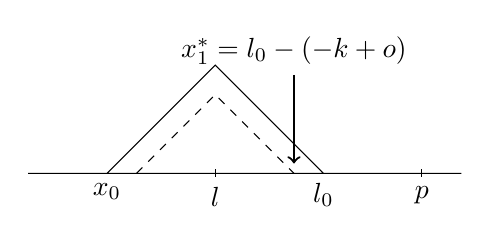
\begin{tikzpicture}[scale=0.5]
          \draw (0,0) -- (11,0) 
          (2,0) node[below] {$x_0$} -- (4.75,2.75) -- (7.5,0) node[below] {$l_0$}; 
          \draw[dashed] 
          (2.75,0) -- (4.75,2) -- (6.75,0); 
          \draw (4.75,0.1) -- (4.75,-0.1) node[below] {$l$}
                (10,0.1) -- (10,-0.1) node[below] {$p$};
          % \draw[->] 
          %       (7,-1) node[below] {$(l_0+o)$} -- (7,-0.25);
          \draw[->, thick] 
                (6.75,2.5) node[above] {\textbf{$x_1^*=l_0-(-k+o)$}} -- (6.75,0.25);
        \end{tikzpicture}
         &
        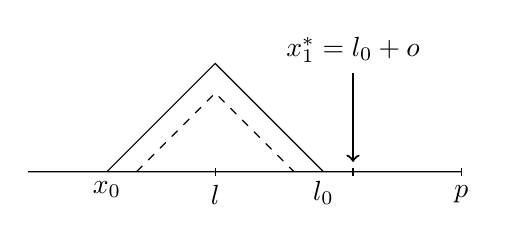
\begin{tikzpicture}[scale=0.5]
          \draw (0,0) -- (11,0) 
          (2,0) node[below] {$x_0$} -- (4.75,2.75) -- (7.5,0) node[below] {$l_0$}; 
          \draw[dashed] 
          (2.75,0) -- (4.75,2) -- (6.75,0); 
          \draw (4.75,0.1) -- (4.75,-0.1) node[below] {$l$}
                (11,0.1) -- (11,-0.1) node[below] {$p$}
                (8.25,0.1) -- (8.25,-0.1) ;
          % \draw[->] 
          %       (8,-1) node[below] {$(l_0-o)$} -- (8,-0.25);
          \draw[->, thick] 
                (8.25,2.5) node[above] {\textbf{$x_1^*=l_0+o$}} -- (8.25,0.25);
        \end{tikzpicture}
         \\
  \mc{1}{l|}{Case 2: $k \geq o$} &  \\
        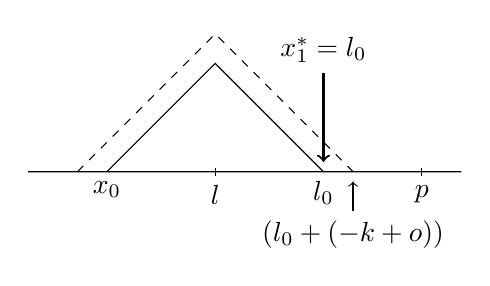
\begin{tikzpicture}[scale=0.5]
          \draw (0,0) -- (11,0) 
          (2,0) node[below] {$x_0$} -- (4.75,2.75) -- (7.5,0) node[below] {$l_0$}; 
          \draw[dashed] 
          (1.25,0) -- (4.75,3.5) -- (8.25,0); 
          \draw (4.75,0.1) -- (4.75,-0.1) node[below] {$l$}
                (10,0.1) -- (10,-0.1) node[below] {$p$};
          \draw[->] 
                (8.25,-1) node[below] {$(l_0+(-k+o))$} -- (8.25,-0.25);
          \draw[->, thick] 
                (7.5,2.5) node[above] {\textbf{$x_1^*=l_0$}} -- (7.5,0.25);
        \end{tikzpicture}
         &
         \\
       \end{tabular}
\caption{Equilibrium costly-scheduling proposals in three cases}\label{f:chiUruEql}
\end{figure}

The legislator's optimal choice depends, in part at least, on the $-k+o$ term. Using the standard notation and spatial assumption used throughout the book, $l_0$ in the figure is that alternative leaving the legislator indifferent vis-\`a-vis the status quo (before netting any other costs). If ignoring leaves the status quo in place, it also adds $-k+o$ to the legislator's utility, and the net value of ignoring must be read through the dashed indifference sets. Whenever the opportunity cost more than counters ignoring cost (i.e., $k<o \leftrightarrow -k+o>0$, as in the figure's case 1), ignoring gives a bonus and therefore dominates rejecting. If the president calibrates a proposal at $x_1 = l_0$---which, in the standard game, prompts acceptance---the legislator is better off ignoring it (thus receiving $x_0$ at the dashed value, which is closer to his ideal point $l$ than the proposal). The president must therefore make further concessions in order to get the proposal accepted (a proposal at $x_1=l_0-(-k+o)$ leaves the legislator indifferent). 

When $k\geq o$ (as in case 2), the dashed line falls beyond the legislator's costless indifference set, and rejecting dominates ignoring. In such case, a proposal at $x_1=l_0$ is accepted.\footnote{This claim assumes that, when indifferent between accepting and rejecting, the legislator chooses the former. Locating the proposal at $x_1=l_0-\epsilon$ ($\epsilon>0$ tiny), as in chapter 2, achieves the same without this assuption, but is less economical in notation.} And in case 3, where only cost $o$ intervenes (and is assumed positive), ignoring dominates accepting, offering the president room to extract welfare from the legislator. Ignoring a proposal at $x_1=l_0$, valued with the dashed line (which, given $0>0$, is contained by the costless indifference set), dominates both accepting and rejecting. With that in mind, an alternative proposal at $x_1=l_0+o$, leaving the legislator indifferent, is still ignored but with fewer executive concessions. 

In sum, unlike the $r=x_1$ institution, urgency authority with costly time and $r=x_0$ never operates in favor of the executive, as the legislator may gain further influence in policy bargaining. Chilean urgency only operates to re-balance executive-legislative policy influence when cost $k$ is large enough to compensate the legislator's opportunity cost. That can be achieved by lowering the size or $o$ or heightening the size of $k$. 

Urgency degree raises $k$

Sending relevant policy (i.e., labeling ``urgent'' an objectively urgent issue) drops the size of $o$

Hence a puzzle: why are `four-week' messages so numerous?
%The latter study quotes the chief of legislative staff describing `four week' notices as merely ``symbolic, exerting no real pressure on Congress'' (p.~117). Similarly, \citet{aleman.navia.UrgChi.2009} see low-degree urgency as ``signals of presidential attention'' (p.~404). (EMM suggests that non-compliance should be concentrated in this category, verify). 
Might they actually bring results? Not speed, but push bills through hurdles. Will pay attention to two observable steps: committee reports, and vote. 




%What if Congress fails to act? Can urgency be ignored? Can a committee report kill the bill or does urgency compell a vote in the floor (law's art.\ 27 ``su discusión y votación en la Cámara requerida deberán quedar terminadas en el plazo'')?




--> Next, discuss Chile in detail. Tie salience to degree of urgency, showing that `Act now' is muche less used. 

--> Hypotheses about div gov: cartel (in one chamber at least) does not have the president on its side, losing key negative agenda control. Makes majority's life much harder. 

--> Connect to frequency of urgency usage; to reports observed and not withing deadline; to roll call votes celebrated. 

--> Regressions on reports

--> Regression on votes?

--> Conclude about the effects of indeterminacy in Chile; announce Brazilian study.

\section{Lit: use for intro and rest for previous section}

The urgency authority has received relatively scant scholarly attention. In a piece putting Chilean executive-legislative relations in perspective, \citet{siavelis.2002} hypothesized urgencies' game-changer potential. Data covers the first Chilean post-transition presidency only, yet revealed just how very frequently urgency messages are sent to Congress: slightly more than one-third of proposals in Congress received some form of urgency, and about 9 out of 10 of urgent bills were executive-initiated. Following semantics, analysis sought to discover if urgent bills, in fact, circulated the steps of the legislative process faster than the rest; whether urgency status also increased the likelihood of bill passage was also investigated. The study found mixed evidence, at best. Among executive bills, consideration of urgent ones had somewhat shorter duration than the rest (medians of 134 and 160 days, respectively), but no palpable difference in success rates is appreciated (64 and 63 percent, respectively). 

The negative finding is partly attributable to not distinguishing urgency degrees (discussed at length in section xx) in the analysis. \citeauthor{aleman.navia.UrgChi.2009}'s \citeyearpar{aleman.navia.UrgChi.2009} systematic study of executive success in Congress in three post-transition presidencies does this, finding some of the evidence sought by Siavelis. Controlling for bill characteristics (such as key policy domains, the chamber of origin, government seat margins, and presidential approval) and clustering errors by legislative year (to capture heterogeneity of grandly changing presidential agenda sizes), different urgency degrees had quite different effects in passage. Higher urgency degrees are significantly associated with increased probability of executive bill passage, but the low degree (which is also much more common, as will be seen) made no statistical difference.

% longer review of aleman and navia
%\citeauthor{aleman.navia.UrgChi.2009}'s \citeyearpar{aleman.navia.UrgChi.2009} systematic study of executive success in Congress in three post-transition presidencies also inspects Chile's urgency authority. Among controls, their equation includes urgency authority usage in the right side. The unit is the individual bill, and the size of the executive agenda varies substantially over the years. Variation is quantitative  (Congress received about 150 presidential bills in each of the first 6 years after 1990, a numbrer that dropped to about 70 in the next 6 years, then climbed to about 100 in the final 4 years of their series) and qualitative, presidents manifesting different propensities to aim at constitutional reform. Of direct relevance are the findings on urgencies. Controlling for key policy domains, chamber of origin, seat margins, and presidential approval, and clustering errors by legislative year, different prioritization reveal quite different effects in passage. `Act now' and `2-week' notices significantly increased the probability of bill passage, but not `4-week' notices. 

The negative finding may also be partly attributable to selection bias: the set of bills receiveing urgent status is not random. Urgent status may, in fact, speed up consideration and increase the odds of passage. But presidents, behaving strategically, were to target for urgency proposals that are markedly different from the rest in exactly those respects, a problem of endogeneity arises. It poses an obstacle to measure urgency authority effects. Like both Siavelis and Alem\'an-Navia, this chapter recognizes the problem but does not confront it methodologically. Until a better identification design is proposed, findings must be taken with a grain of salt. Correlations of the urgency authority with committee reports and with floor votes are offered in this chapter in the hope of helping pave the way for a solution. 

%The relevant quantity of interest is whether the use of the urgency authority affects bill passage (success, speed, amendments, and so forth) compared to the same bill with no urgency attached. The fundamental problem of causal inference is immediately evident. The executive presumably targets bills for urgency strategically, so that the selection mechanism cannot be assumed random. If, for example, more complex and divisive legislation takes longer, is likelier to fail and likelier to be tagged urgent, separating effects requires more subtle methods than used up to now.




\section{The data}

The data analyzed here is from the C\'amara de Diputados' web page (\url{www.camara.cl}), a remarkably informative and up-to-date primary source. It offers detailed reports with bills' general traits: who initiated it, when, in what chamber, what it deals with, its status, and so forth. The report also lists and dates the proposal's milestones in transit through the meanders of the bicameral legislative process: committee referral, committee reports to the plenary, floor discussion and voting, navette to the other chamber, etc. Of direct relevance, all urgency messages that bills received are listed chronologically.

\begin{table}
\begin{center}
\begin{tabular}{lrrrrrr}
Coalition   & 1990--94 & 1994--98 & 1998--2002    & 2002--06 & 2006--10 & 2010--14 \\ \hline
\mc{7}{l}{\emph{~~C\'amara de Diputados}} \\
President's & 60       & 58       & 58            & 53       & 51       & 50       \\
Opposition  & 40       & 42       & 42            & 48       & 47       & 48       \\
Regional    &          &          &               &          & 3        & 2        \\ \hdashline
Total       & 100      & 100      & 100           & 100      & 100      & 100      \\ \hline
\mc{7}{l}{\emph{~~Senate}} \\
President's & 48       & 46       & 50            & 50       & 55       & 45       \\
Opposition  & 52       & 54       & 50            & 50       & 45       & 55       \\ \hdashline
Total       & $100^*$  & $100^*$  & $100^{*\dagger}$ & 100      & 100      & 100      \\ \hline
\mc{7}{l}{\footnotesize{Notes: $^*$ vacant seats dropped; $^\dagger$ margin varied above and below 50/50 due to vacancies.}}

\end{tabular}
\caption{The president's status in Congress. Percent seats controlled by electoral lists in each chamber. Between 1990 and 2010, the president's and opposition lists were Concertación and Alianza, respectively; they switched after 2010. The regional list includes splinters from each major list (Christian Democrats and UDI members). Source: prepared by the author with information from the C\'amara's web page at \protect\url{www.camara.cl} (some data kindly shared by Guillermo Rosas).}\label{t:congressSeats}
\end{center}
\end{table}

The web page was scraped in November 2014 to obtain every record (bolet\'in) for proposals made between March 1998 and February 2014.\footnote{An inquiry was sent to the congressional staff in Oct.\ 2014 about the existence of an official API ot FTP site where this well-structured data could be downloaded en bloc. There was no response, so an automated script was prepared to download the data. The web page is javascript-rich, an obstacle that \texttt{Python}'s Selenium library was capable of overcoming to put together the bits and pieces of the scraping process. A commented version of the script, and the data will be posted online upon publication. Data analysis was done with a multiplicity of \texttt{R}'s libraries.} The period fully covers the tenures of two Senates, four C\'amaras de Diputados, and two presidencies; the first two years cover the end of the Frei presidency). Earlier years antedate the internet, and data completeness remains to be verified. As reported in Table \ref{t:congressSeats}, with differences in margin, the president's coalition was always in control of the lower chamber; yet controlled senate majorities only between 2006 and 2010 (the first Bachelet administration). Given party coalition voting unity since the return to democracy \citep{carey.2002,aleman.saieg.coalUnityChile.2007}, these are good indicators of the executive's legislative support in Congress. Margins above 50 percent guarantee adequate support in most except subsets of legislation---constitutional reforms require two-thirds votes, constitution-interpreting laws three-fifths, and organic laws four-sevenths (translation?). 

% latex table generated in R 3.1.2 by xtable 1.7-4 package
% Wed Feb  4 17:24:48 2015
\begin{table}
\centering
\begin{tabular}{rrrrr|r}
      & 1998--2002 & 2002--2006 & 2006--2010 & 2010--2014 & 1998--2014 \\ \hline
 Act now             & 5  & 6  & 3  & 4  & 4 \\ 
 2-week notice       & 16 & 14 & 9  & 23 & 16 \\ 
 4-week notice       & 29 & 22 & 13 & 12 & 17 \\ \hdashline
 Shorten deadline    & 2  & 2  & 2  & 4  &  3 \\ 
 Extend deadline     & 29 & 33 & 41 & 43 & 39 \\ \hdashline
 Withdraw (act now)  & 1  & 2  & 2  & 2  &  2 \\ 
 Withdraw (2-week)   & 7  & 10 & 14 & 8  & 10 \\ 
 Withdraw (4-week)   & 10 & 11 & 17 & 3  & 10 \\ \hline
 Total messages      & 100 & 100 & 100 & 100 & 100 \\ 
(N)                  & (1,268) & (1,881) & (4,941) & (5,643) & (13,733)\\ \hline
 Senate status       & \emph{tied} & \emph{tied} & \emph{gov.} & \emph{opp.} & \\
\end{tabular}
\caption{Chilean urgency message types and relative frequencies}\label{t:freqUrg}
\end{table}

Table \ref{t:freqUrg} offers a summary of urgency messages in the dataset. The sheer number of urgency messages that presidents sent is appaling, 13,733 in the 16-year period, nearly 72 monthly on average. The number of messages has risen sharply in each of four subsequent four-year Legislatures reported. Bachelet's first presidency (2006--2010) is responsible for the largest hike, nearly tripling urgency message incidence (the monthly average surpassing 100) compared to the previous Legislature, which ended the Lagos presidency. Not all messages are original urgencies, though. Nearly two-thirds were messages shortening or extending the deadline, and messages withdrawing the urgency status. And given that the urgency authority compels action by the chamber receiving the message, accelerating a bill in Congress would require one original urgency message for each step of the bicameral legislative process---up to four, if the bill goes to conference. Focus on original urgency messages first (the top table rows) reveals how `Act now' notice frequency (4 percent of messages in the period) was one-quarter the frequency of `two' and `four week' messages (16 and 17 percent, respectively). And deadline changes (the middle table rows) normally involved a time extension for bill consideration, but 3 percent of messages actually made urgency more rigorous. And, with variance, urgency withdrawals were quite common too, representing one-third of messages issued by Bachelet.   

% verify numbers in chillBill.r (above xtable command)
\begin{table}
\centering
\begin{tabular}{lrrr}
                                &  by           &  by          &    by      \\
Bills                           &  legislators  &  president   &    ~~~~either  \\ \hline
introduced                      &        5,533  &       1,469  &     7,002  \\
as \%                           &    \emph{79}  &   \emph{21}  & \emph{100} \\ \hdashline
passed                          &          404  &       1,067  &     1,471  \\
as \%                           &    \emph{27}  &   \emph{73}  & \emph{100} \\
as \% of introduced             &     \emph{7}  &   \emph{73}  &  \emph{21} \\ \hdashline
declared urgent (at least once) &          351  &       1,016  &     1,367  \\
as \%                           &    \emph{26}  &   \emph{74}  & \emph{100} \\
as \% of introduced             &     \emph{6}  &   \emph{69}  &  \emph{20} \\ \hdashline
declared urgent \& passed       &          167  &         762  &       929  \\
as \%                           &    \emph{18}  &   \emph{82}  & \emph{100} \\
as \% of declared urgent        &    \emph{48}  &   \emph{75}  &  \emph{68} \\ \hline
\end{tabular}
\caption{Bills, laws, and the urgency authority 1998--2014}\label{T:billDescriptives}
\end{table}

About seven thousand bills were introduced to Congress in the period, 412 yearly on average in Table \ref{T:billDescriptives}. The table distinguishes legislator from executive proposals. Presidents introduced one bill for every four by members of Congress (79 vs.\ 21 percent). In terms of success rates, however, branch asymmetry inverts, a member turning one proposal into law for every three by a president (27 vs.\ 73 percent). And while the success rate of members of the Chilean Congress was dismal (7 percent), they still managed to add four hundred laws in the period due to the sheer volume of proposals made. It is remarkable that one of every five bills introduced in the period received at least one original urgency message. A total of 1,367 legislative proposals deemed urgent suggests a rather lax definition of urgency by Chilean presidents. Note the closeness of the relative figures in the second (urgency) and third (passed bills) sets of table rows. The subset of urgent bills overlaps to a very large extent with the subset of bills passed. In other words, urgency correlates strongly with success: the passage rate of members' bills declared urgent skyrocketed to 48 percent, up from 7 percent altogether (the difference is small for executive bills). It is tempting to conclude that urgency makes bills likelier to pass. But the reverse may also hold, proposals with better prospects in Congress strategically receiving the bulk of urgency messages---the problem of selection bias discussed above \citep[cf.][]{jacobson.kernell.1983}. 

\begin{table}
\begin{center}
\begin{tabular}{rrr}
Number of &      Bill &     \\
messages  & frequency &  ~~~~~~~~\% \\ \hline
%None              &  5635     &     \\
1                 &  215      &  \emph{16}   \\
2                 &  244      &  \emph{18}   \\
3                 &  145      &  \emph{11}   \\
4                 &  115      &  \emph{8}    \\
5                 &  104      &  \emph{8}    \\
6-10              &  236      &  \emph{17}   \\
11-20             &  185      &  \emph{14}   \\
21-40             &  99       &  \emph{7}    \\
41-71             &  24       &  \emph{2}    \\
Total             & 1,367     & \emph{100}   \\ \hline
\end{tabular}
\caption{Urgent bills classified by number of urgency messages received}\label{T:billFreqByNurg}
\end{center}
\end{table}

More interesting patterns in urgency authority usage are discernible in bill histories. The size of the subset of bills receiving one or more urgency messages conveys a minimalist perspective of the urgency authority. As shown in table \ref{T:billFreqByNurg}, most bills in this subset (84 percent) in fact received numerous such messages, and a substantial number (40 percent) received between 6 and 71 urgency messages. This raises another puzzle for research. Are presidents reiterating urgency messages because of Congressional inaction? Extending the deadline may help the president save face when it is imminent that an urgency message has been ignored. Or are presidents micro-managing select-bill consideration in committee, monitoring a report's progress and sending recommendations along with a message extending the deadline? The source indicates the arrival of presidential messages but does not include their actual contents nor those of committee reports. Archival research to retrieve those documents would do wonders in answering these questions. 

%A bicameral process operating on a single-round navette \citep{tsebelis.money.1997}---bills migrate from originating to revising chamber, back to originating if amended, and finally to conference if inter-cameral differences persist---offers, at most, four clear instances for repeated urgency authority use. Yet, as table \ref{T:billFreqByNurg} reports, nearly half of urgent bills (47 percent) received five messages or more. A handful of bills received several dozen messages! 

\begin{figure}
\begin{center}
 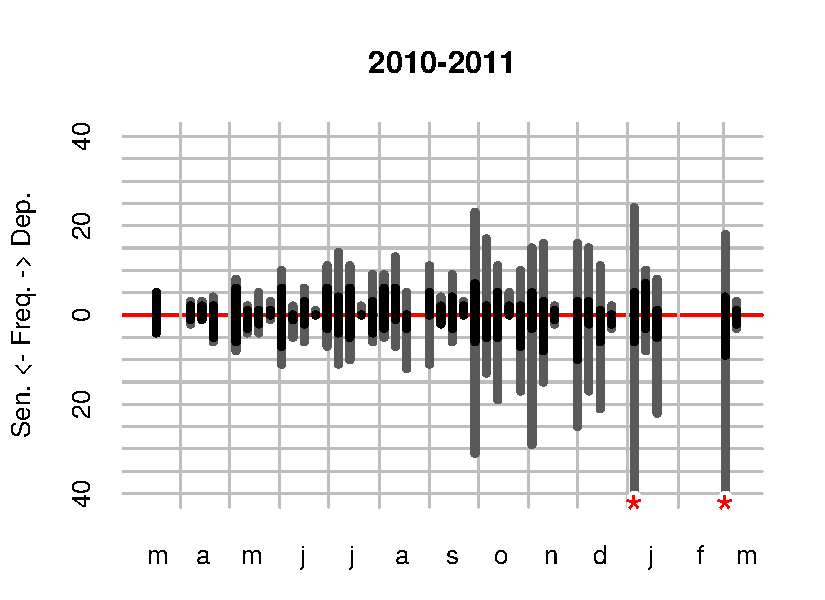
\includegraphics[width=.65\columnwidth]{../graphs/urgenciasHistog2010.pdf}
\begin{tabular}{cccc}
    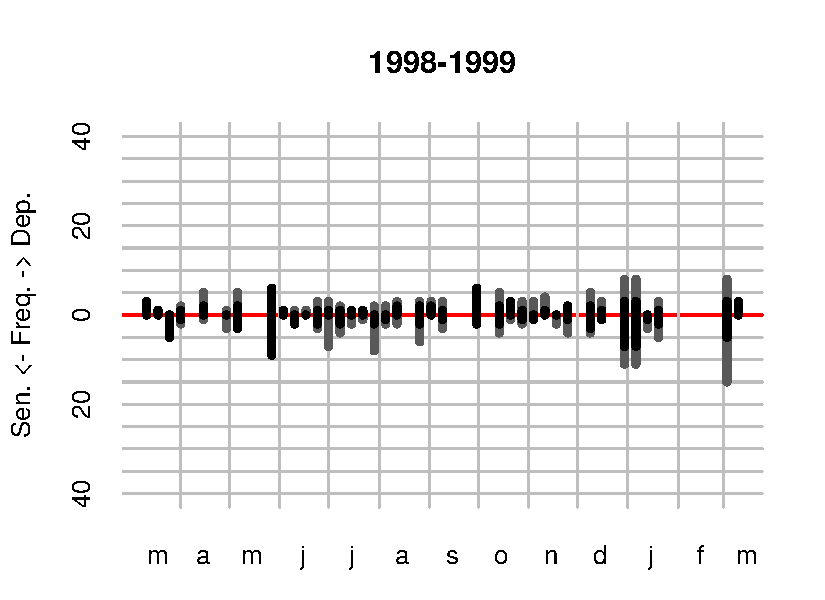
\includegraphics[width=.22\columnwidth]{../graphs/urgenciasHistog1998.pdf} &
    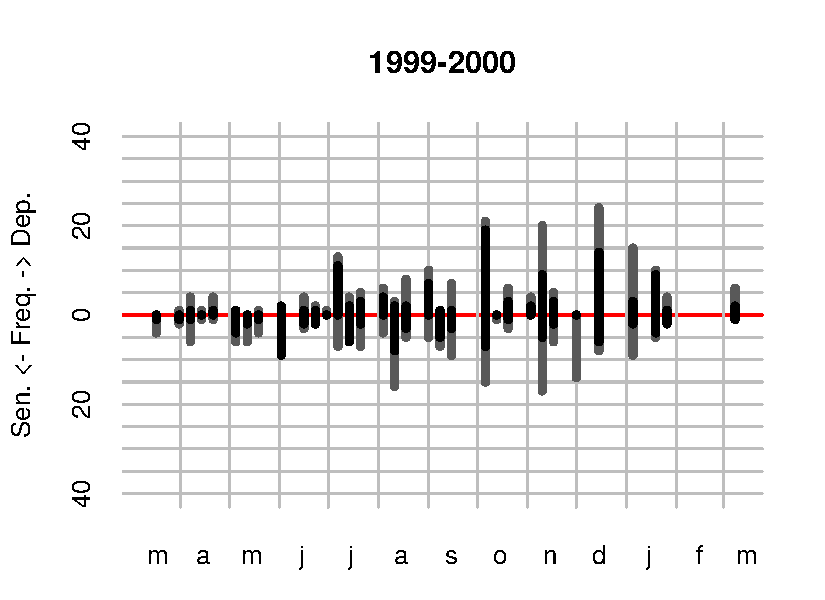
\includegraphics[width=.22\columnwidth]{../graphs/urgenciasHistog1999.pdf} &
    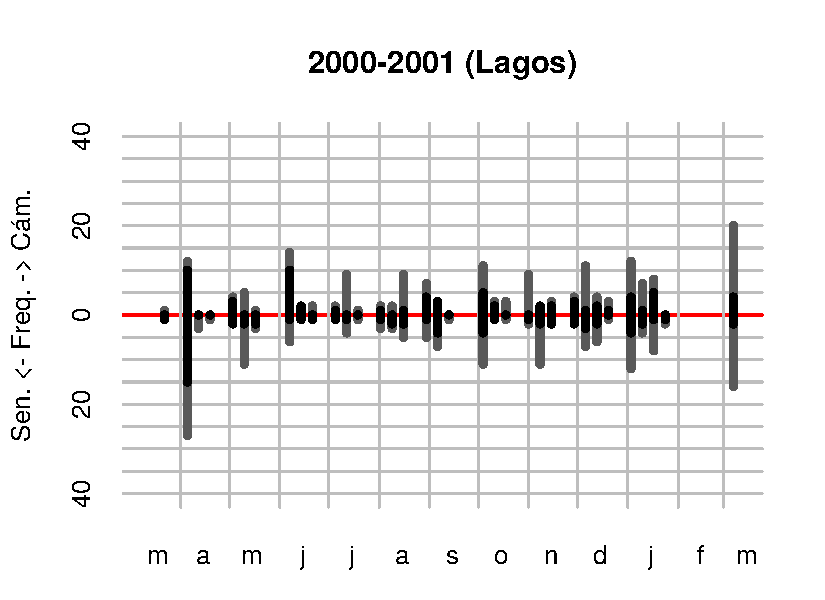
\includegraphics[width=.22\columnwidth]{../graphs/urgenciasHistog2000.pdf} &
    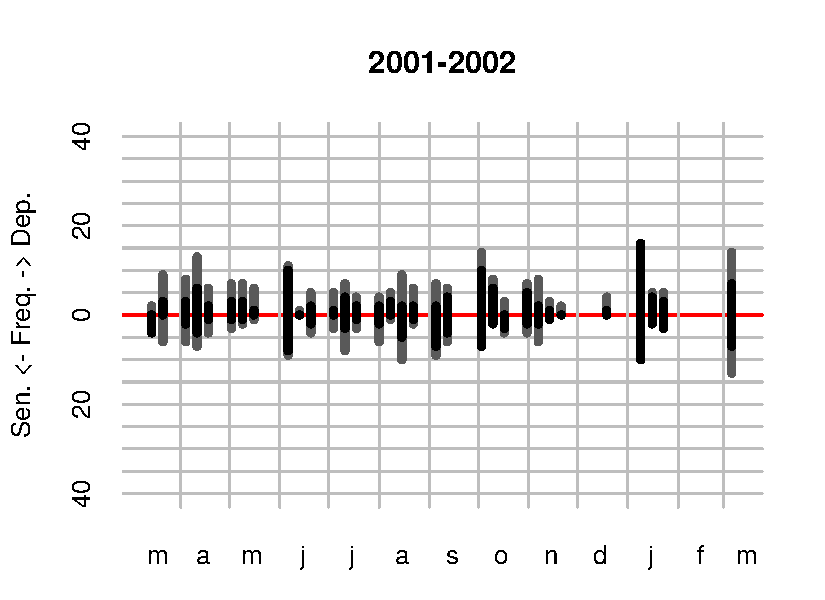
\includegraphics[width=.22\columnwidth]{../graphs/urgenciasHistog2001.pdf} \\
    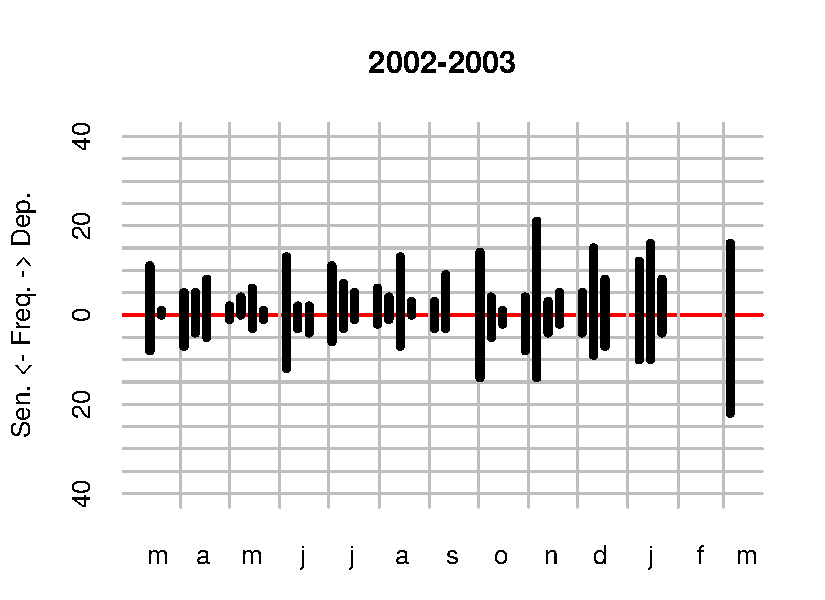
\includegraphics[width=.22\columnwidth]{../graphs/urgenciasHistog2002.pdf} &
    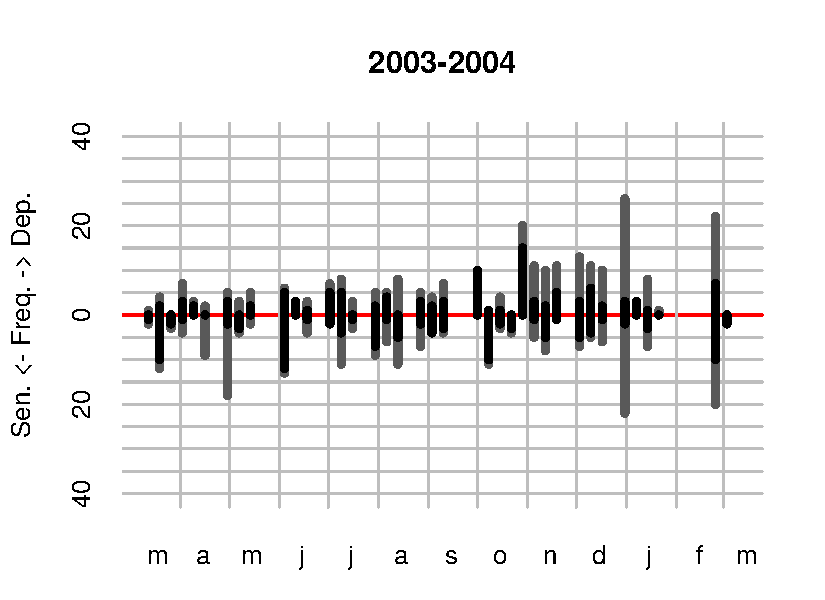
\includegraphics[width=.22\columnwidth]{../graphs/urgenciasHistog2003.pdf} &
    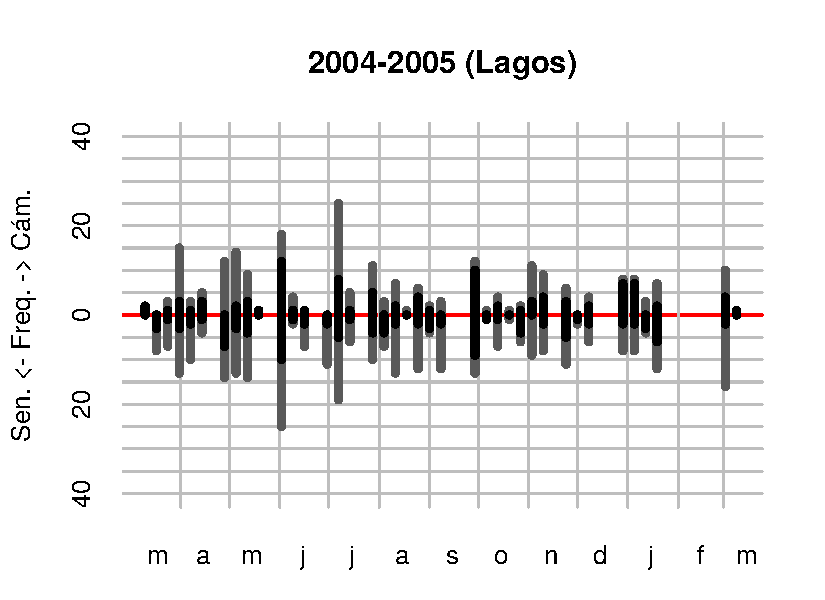
\includegraphics[width=.22\columnwidth]{../graphs/urgenciasHistog2004.pdf} &
    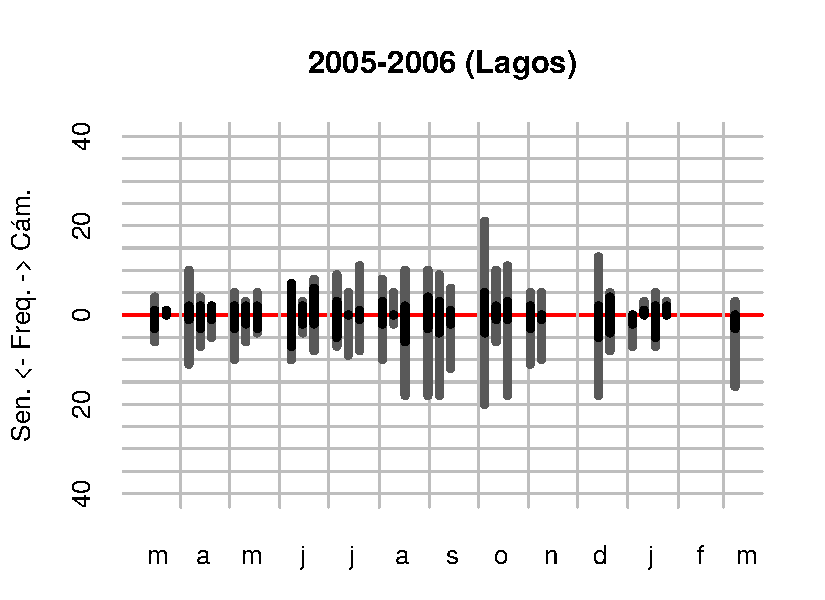
\includegraphics[width=.22\columnwidth]{../graphs/urgenciasHistog2005.pdf} \\
    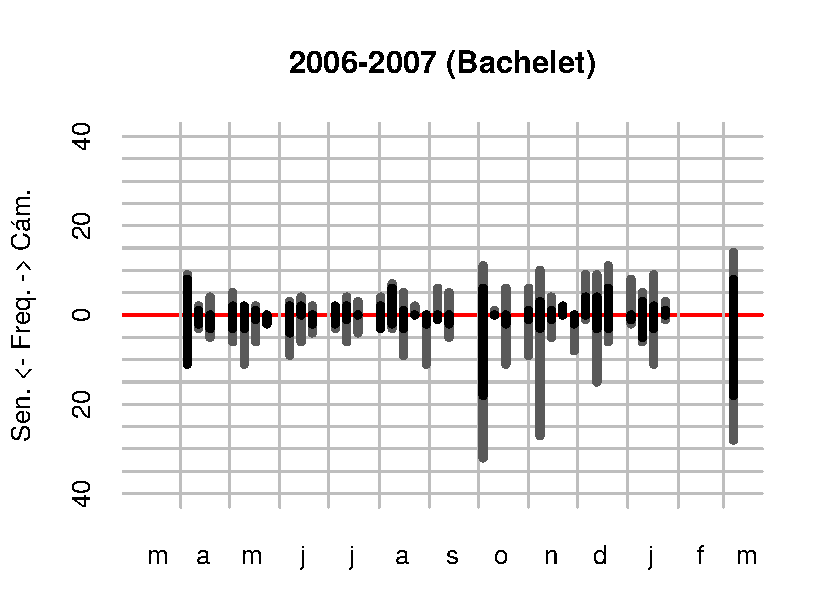
\includegraphics[width=.22\columnwidth]{../graphs/urgenciasHistog2006.pdf} &
    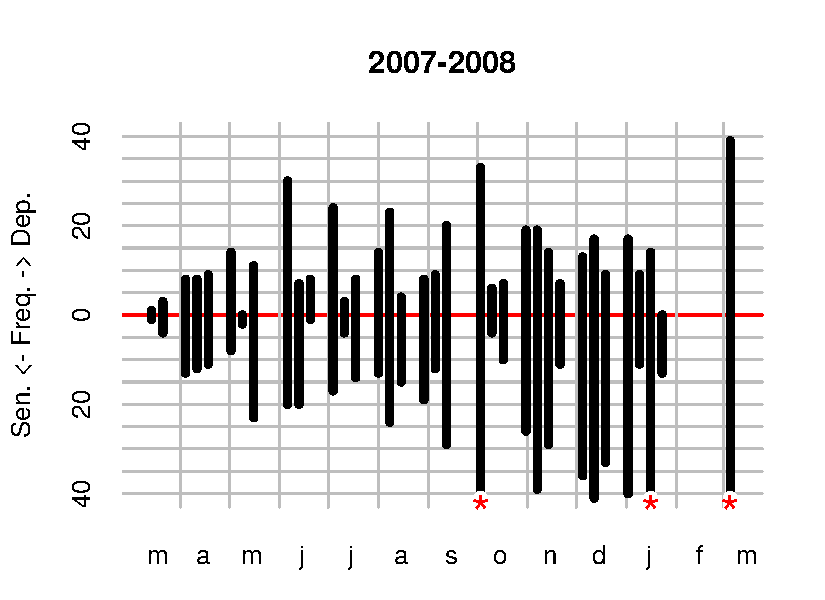
\includegraphics[width=.22\columnwidth]{../graphs/urgenciasHistog2007.pdf} &
    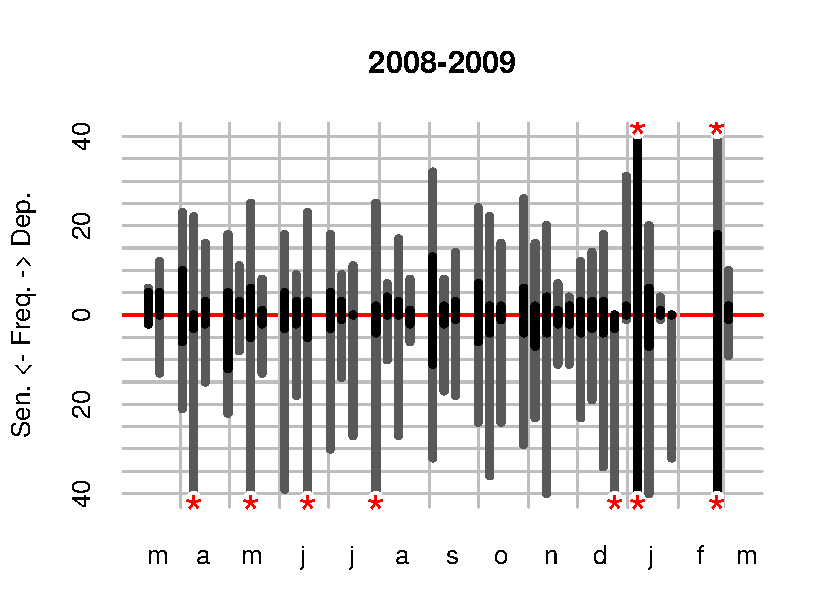
\includegraphics[width=.22\columnwidth]{../graphs/urgenciasHistog2008.pdf} &
    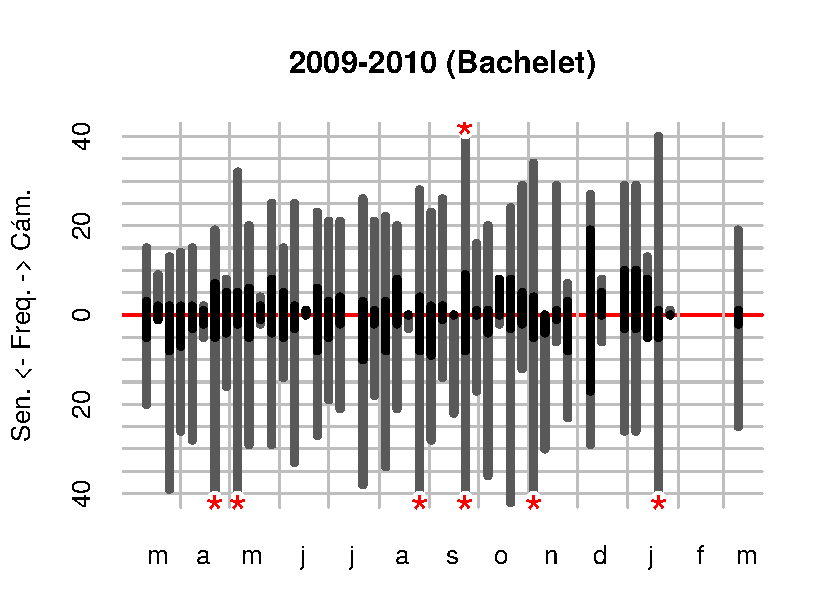
\includegraphics[width=.22\columnwidth]{../graphs/urgenciasHistog2009.pdf} \\
    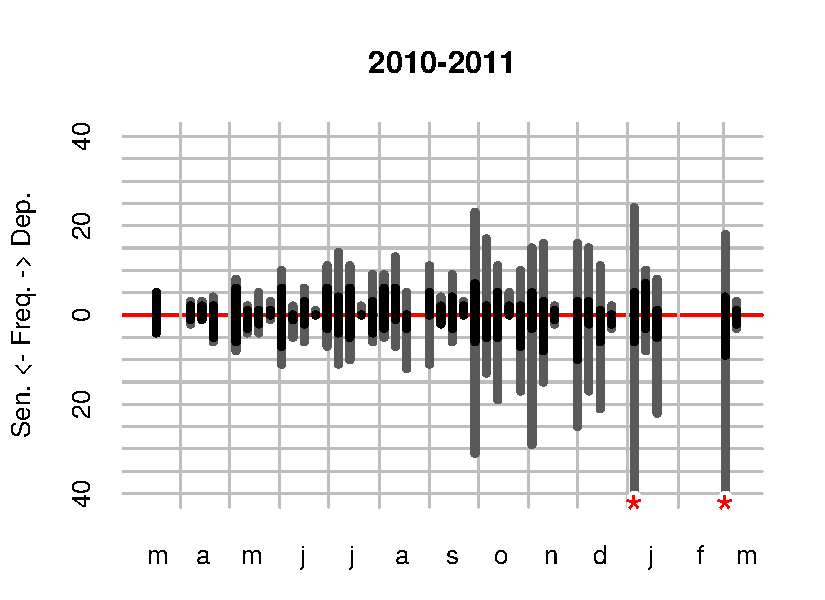
\includegraphics[width=.22\columnwidth]{../graphs/urgenciasHistog2010.pdf} &
    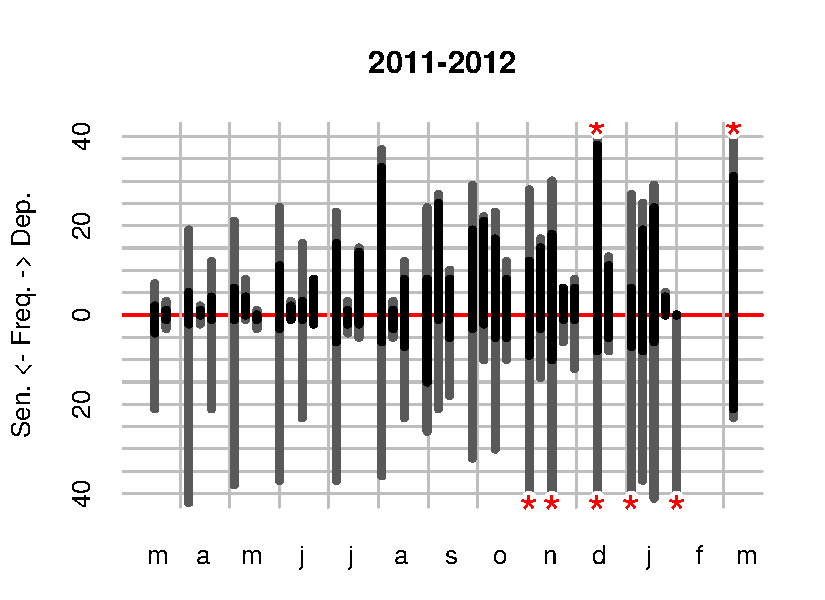
\includegraphics[width=.22\columnwidth]{../graphs/urgenciasHistog2011.pdf} &
    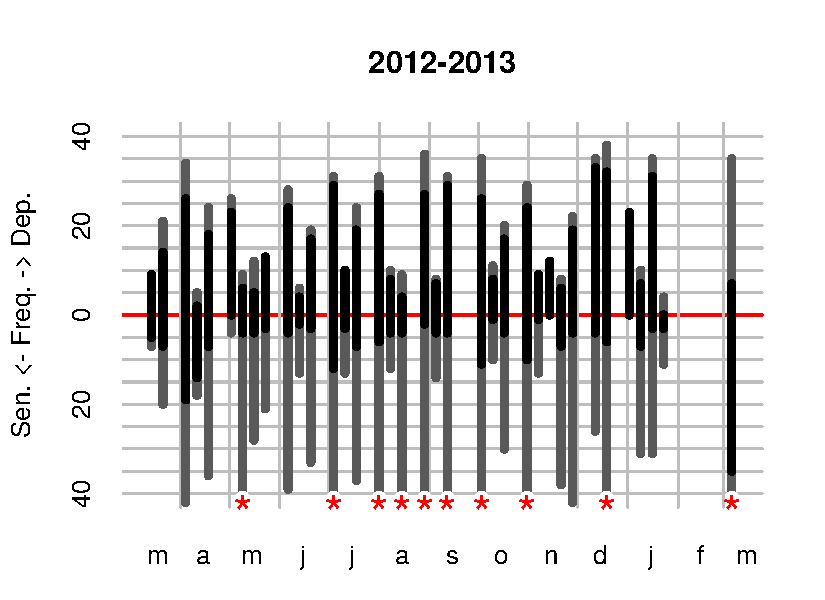
\includegraphics[width=.22\columnwidth]{../graphs/urgenciasHistog2012.pdf} &
    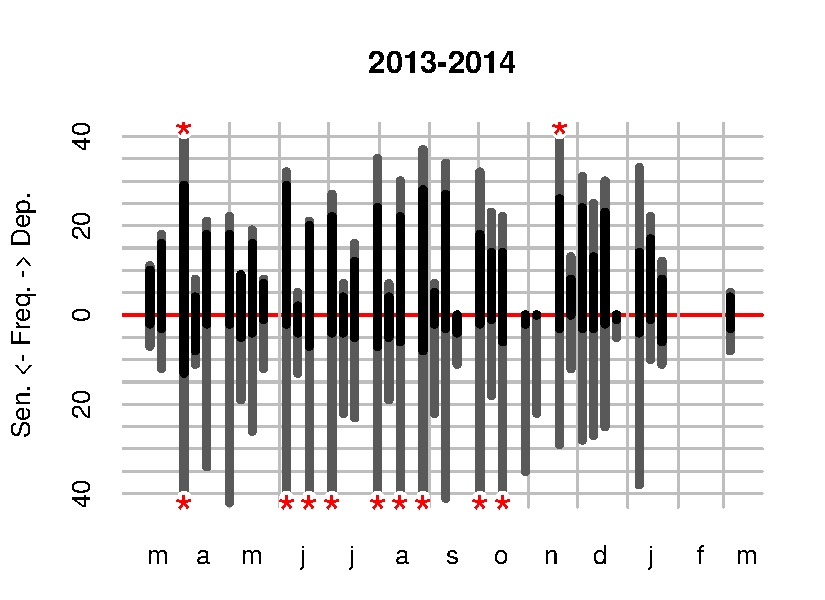
\includegraphics[width=.22\columnwidth]{../graphs/urgenciasHistog2013.pdf} \\
\end{tabular}
  \caption{Weekly urgencies by legislative year. Deputies histogram above, Senate below the zero line. Asterisk atop column indicates off-the-chart urgency message frequency. Source: prepared with data from the Chilean Congress.}\label{f:depvarHistog}
\end{center}
\end{figure}

\begin{figure}
\begin{center}
    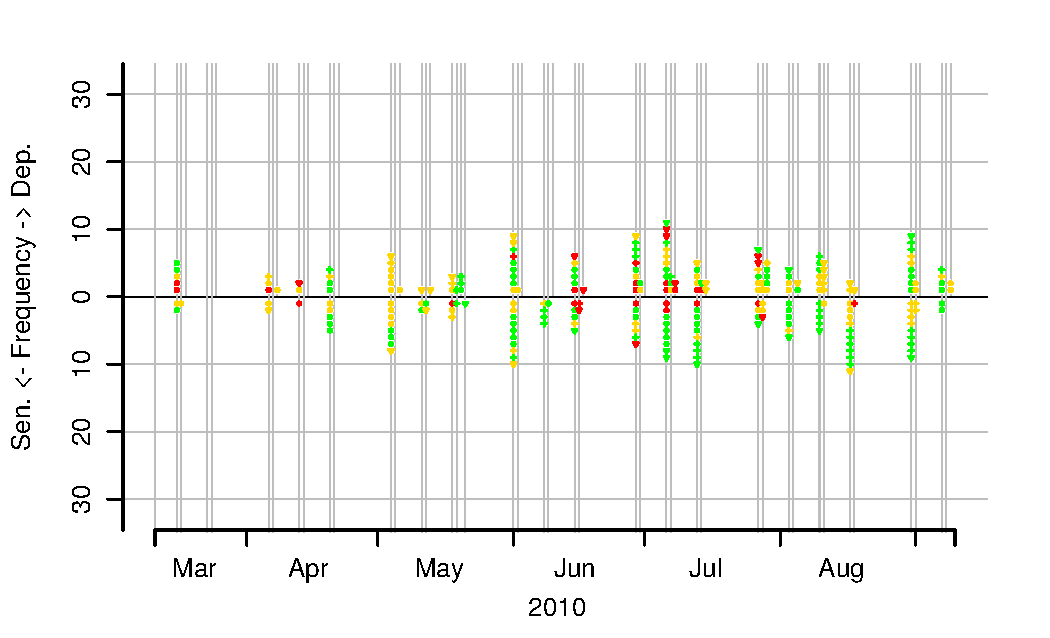
\includegraphics[width=\columnwidth]{../graphs/urgencias2010-1.pdf} \\
    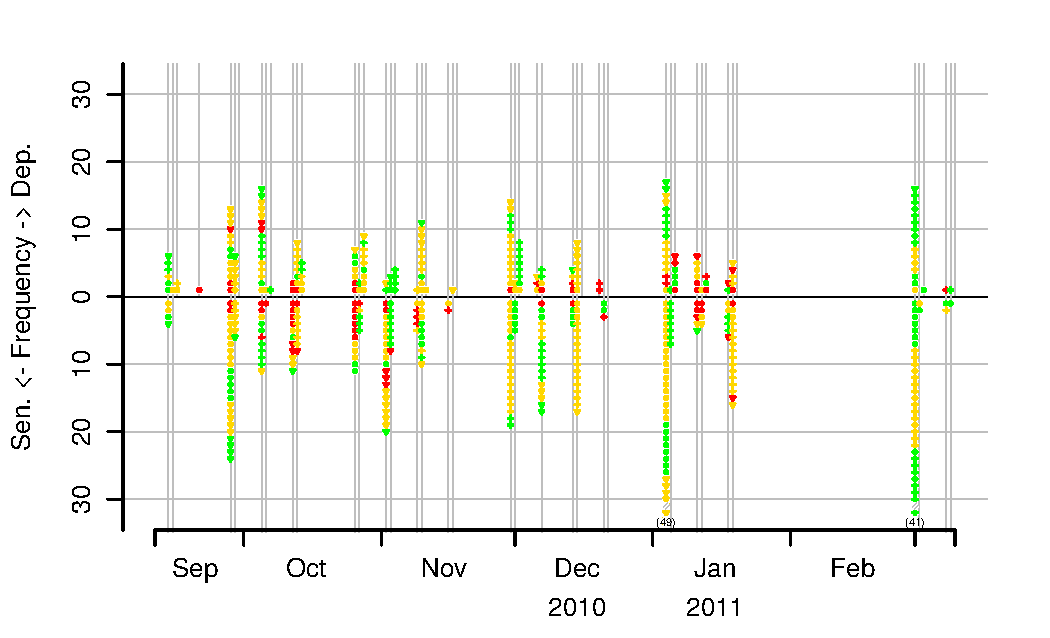
\includegraphics[width=\columnwidth]{../graphs/urgencias2010-2.pdf} 
  \caption{Urgencies in one legislative year. Deputies and Senate data above and below the zero line, respectively. Vertical grey lines indicate that a session took place. One point for each urgency message, a circle for a newly declared urgent bill, a plus sign for an urgent bill with new deadline, an inverted triangle for a retired urgency. Point color indicates the urgency deadline, red for 3/6 days, yellow for 10/15 days, green for 30 days. Parentheses atop columns indicate off-the-chart urgency message frequency.}\label{f:depvar}
\end{center}
\end{figure}

Another puzzle arises when inspecting urgent member-initiated proposals. If the urgency authority, despite the lack of institutional teeth, exerts pressure (through cost $k$) on legislators, the abundance of urgency messages observed poses a genuine scheduling problem for legislators and their parties. Figure \ref{f:depvarHistog} gives an idea of this phenomenon, reporting the number of weekly urgency messages received by the chambers of Congress (each plot is made of two, super-imposed histograms, one for C\'amara and one for Senate messages). Not taking the February Summer break into account (when Congress rarely convenes),\footnote{Three February weeks with urgency messages are retained in the count and denominator.} less than one in three weeks in the period were free of urgency messages. The executive sent 7.6 weekly messages on average to the C\'amara de Diputados, and 10.5 to the Senate. And Figure \ref{f:depvar}, reporting sessions' urgency message count and type in legislative year 2010--11, shows large numbers of original urgencies relative to deadline changes and urgency withdrawals. 

\begin{table}
\begin{center}
\begin{small}
\begin{tabular}{lrrrrrrrr}
                         &  \mc{8}{c}{Percent Concertaci\'on sponsors} \\
Urgency raised by        &  0\%      &  1--25\%  &  26--50\%  &  51--75\%  &  76--99\%  &  100\%      &  All         &  N \\ \hline
Concertaci\'on presidents& \emph{21} & \emph{3}  & \emph{10}  & \emph{15}  & \emph{13}  & \emph{39}   &  \emph{100}  &  230 \\
Right president          & \emph{26} & \emph{4}  & \emph{18}  & \emph{12}  & \emph{12}  & \emph{26}   &  \emph{100}  &  121 \\
\end{tabular}
\caption{Sponsorship of urgent member bills. Entries are relative frequencies of Concertaci\'on sponsors among bills declared urgent by presidents elected by a given list. The first entry reports that 21 percent of bills declared urgent by a Concertaci\'on president had not a single sponsor elected by that list; and so forth.}\label{T:sponsorsOfUrgBills}
\end{small}
\end{center}
\end{table}

Saturating the agenda with urgent executive bills inevitably leaves precious little time to consider members' pet projects.\footnote{\citet{berrios.gamboa.fiscChile.2006} quote minister ``Para evitar entorpecer el funcionamiento de Congreso, el Ejecutivo procura no tener, al mismo tiempo, más de 10 proyectos con urgencia en cada una de las Cámaras (entrevista Carmona)'' (fn.~25), are quite optimistic about this self-restraint. Presidents better descibes as run amok in urgency authority usage...} In such circumstances, the urgency authority gives presidents another asset for vote-buying, granting members' projects urgent status in exchenge for supporting presidential proposals short of votes in the chamber. Table \ref{T:sponsorsOfUrgBills} suggest this possibility: controlling for the percentage of signatures by legislators belonging to Concertaci\'on parties in the proposal reveals that presidents often granted urgent status to opposition bills. Of member bills declared urgent by Concertaci\'on presidents (1998--2010), 21 percent fell in this category, and 26 percent by the right-of-center president (2010--2014). This is yet another promising area for future research.


%   Cámara  
% ##########
%    Min. 1st Qu.  Median    Mean 3rd Qu.    Max. 
%   0.000   0.000   4.000   7.602  11.000  85.000 
%   Senado  
% ##########
%    Min. 1st Qu.  Median    Mean 3rd Qu.    Max. 
%    0.00    0.00    5.00   10.49   14.00   97.00 


% \begin{sidewaysfigure}
% \begin{center}
%     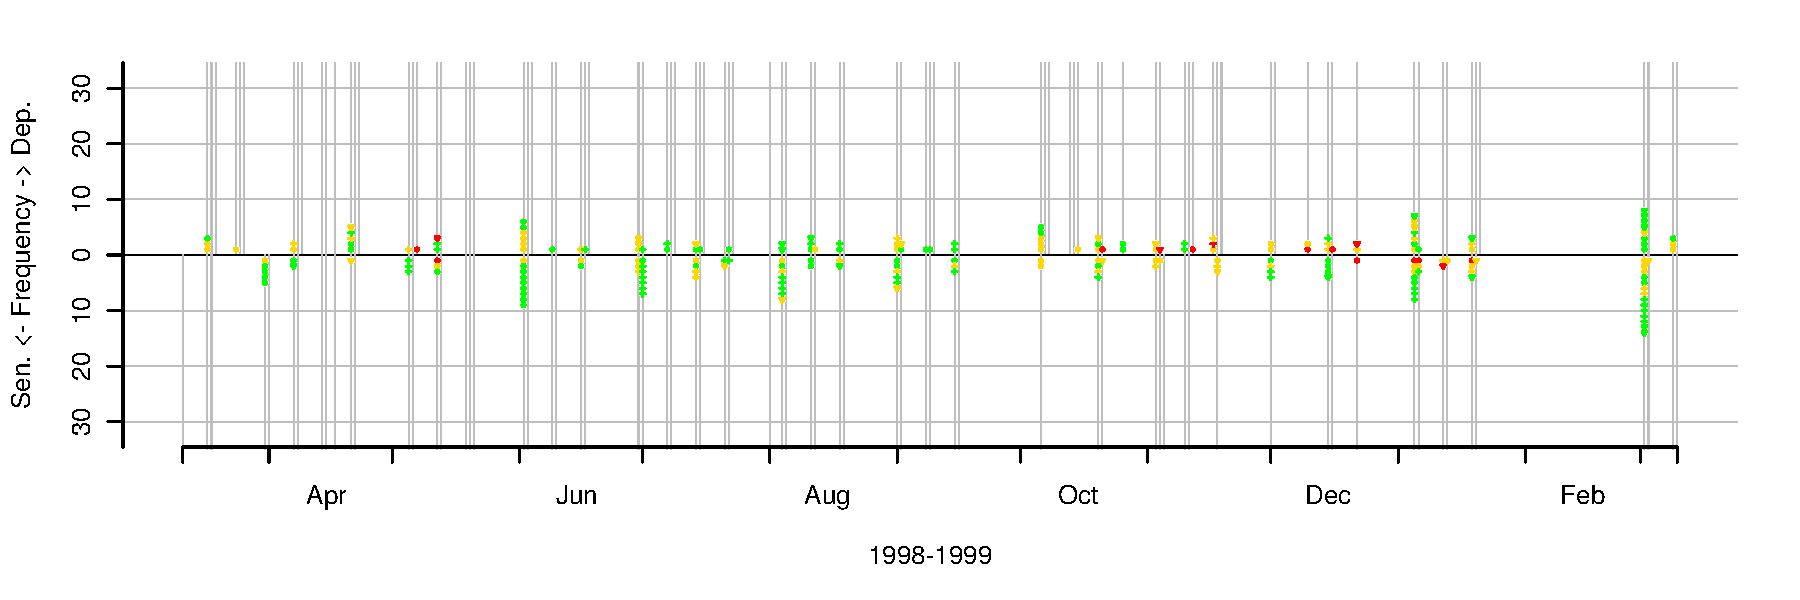
\includegraphics[width=\columnwidth]{../graphs/urgencias1998.pdf} \\
%     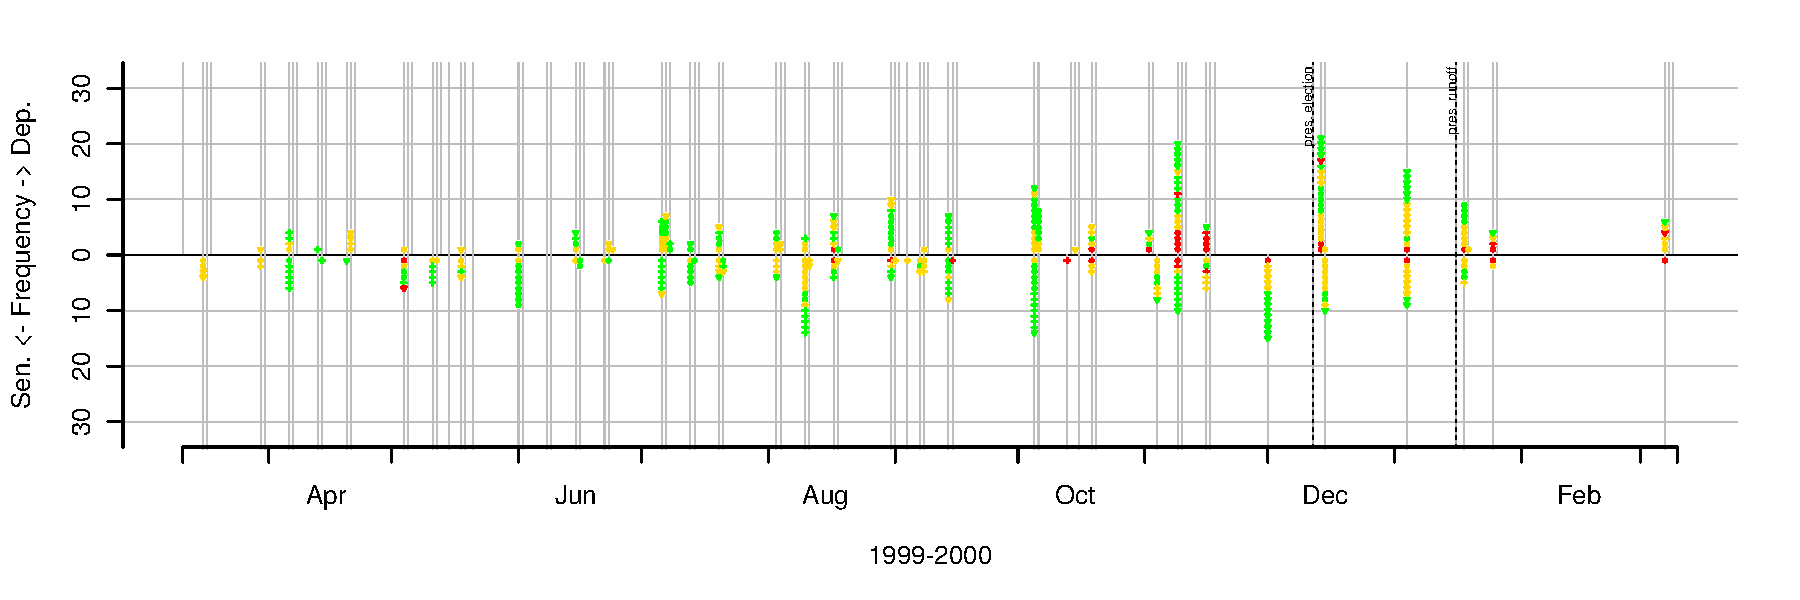
\includegraphics[width=\columnwidth]{../graphs/urgencias1999.pdf} 
%   \caption{Urgencies by legislative year. Deputies and Senate histograms above and below the zero line, respectively. Vertical grey lines indicate that a session took place. One point for each urgency message, a circle for a newly declared urgent bill, a plus sign for an urgent bill with new deadline, an inverted triangle for a retired urgency. Point color indicates the urgency deadline, red for 3/6 days, yellow for 10/15 days, green for 30 days. Parentheses atop columns indicate off-the-chart urgency message frequency.}\label{f:depvar}
% \end{center}
% \end{sidewaysfigure}

% \begin{sidewaysfigure}\ContinuedFloat
% \begin{center}
%     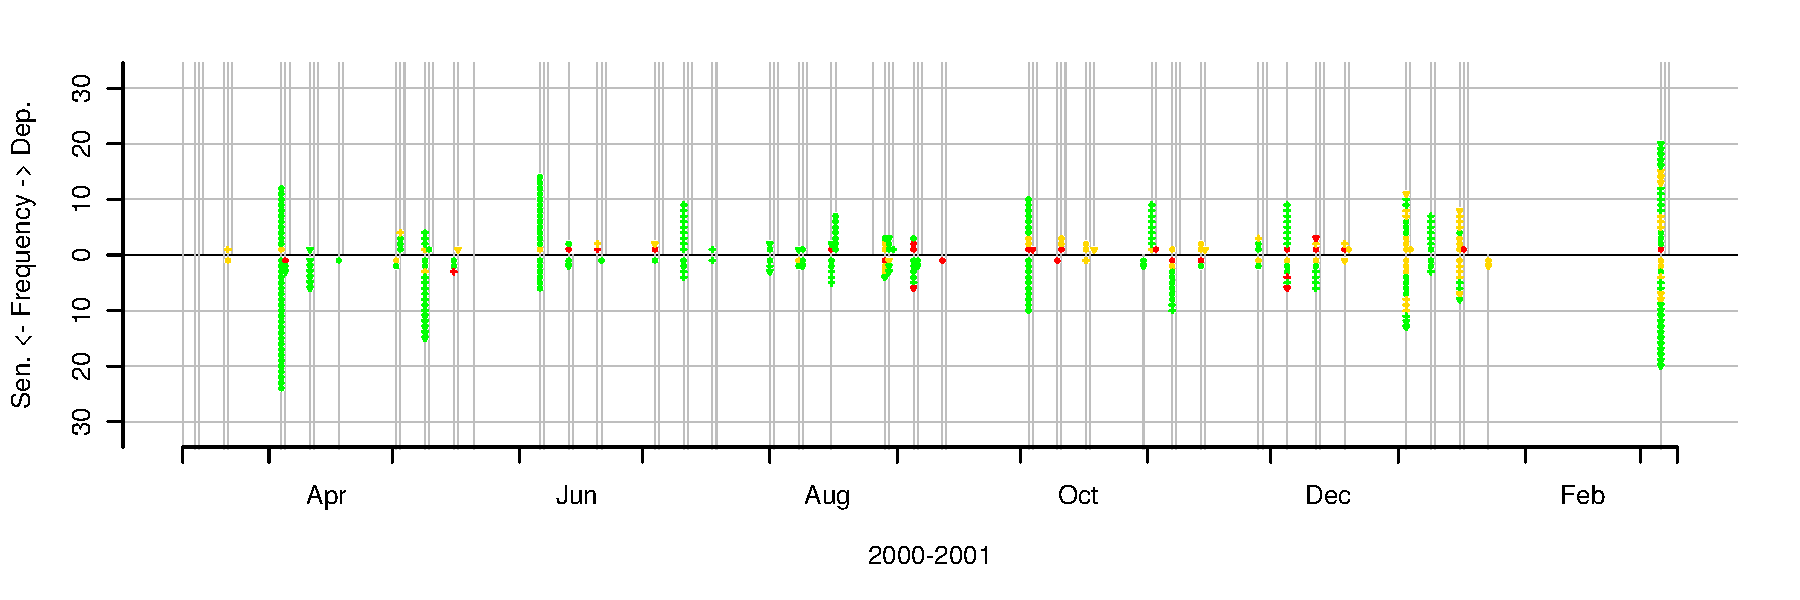
\includegraphics[width=\columnwidth]{../graphs/urgencias2000.pdf} \\
%     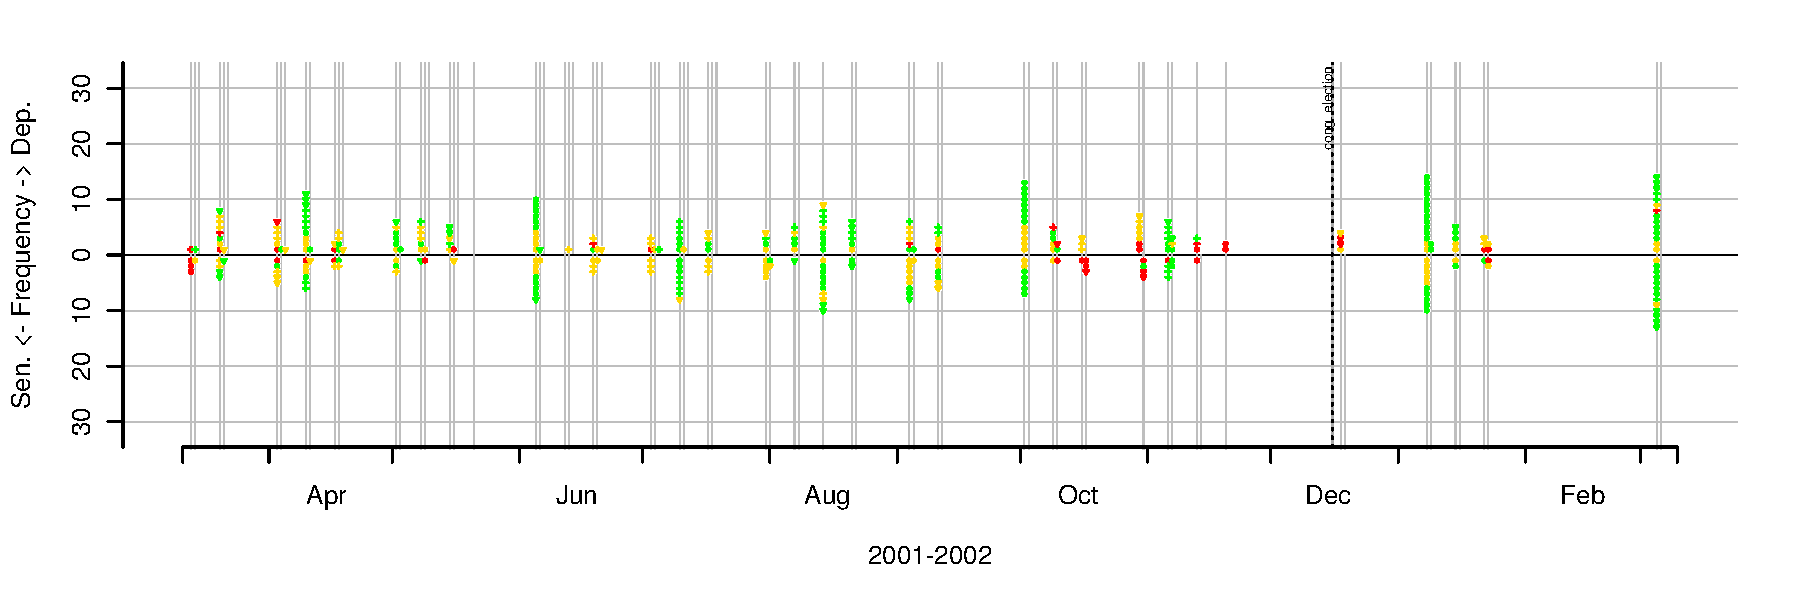
\includegraphics[width=\columnwidth]{../graphs/urgencias2001.pdf} 
%   \caption{Urgencies by legislative year (cont.)}\label{f:depvar}
% \end{center}
% \end{sidewaysfigure}

\section{Committee reporting}

Reporting proposals to the floor are observable steps in the bill histories collected. Report contents are unfortunately unavailable, but the committee who drafted the report in question and the report's date are included. It is a step of the legislative process worth inspecting in search for effects of the urgency authority. Unless the floor votes an exception unanimously, every bill in Chile is referred to a standing or special committee upon first introduction to each chamber. 

With the exception of bills exempt from committee referral, or that have already been reported and await subsequent steps for floor consideration, a committee report (or several, in case of multiple referrals) should follow an urgency message. Moreover, taking urgency degrees into consideration, the finer expectation that bill reporting should occur \emph{before} the given deadline arises. 

This section analyzes bill histories to detect whether or not a report follows an urgency message, and whether or not it occurs in a timely manner. Failure to observe the report is strong evidence of inconsequential urgency authority.  

No explicit discharge procedure could be found in the Reglamento, but presumably is the same---unanimous consent---to consider a bill without prior committee referral. Absent a consequential urgency authority, this plays in favor of turning committees into formidable gatekeepers in their jurisdiction's policy domain: failure to draft a report prevents any proposal from progressing towards floor consideration \citep{cox.mccubbins.1993,fenno.1973,shepsle.weingast.1987}. Consequential urgency authority, however, undermines committees' negative agenda power, by forcing them to open the gates of bills they would rather not let the floor consider. 

The Hacienda (Finance) committee has special status in the Chilean committee system and deserves attention. Hacienda stands apart from other standing committees as it has jurisdiction over every bill authorizing spending in any domain. So a proposal restricting eligibility to certain labor benefits among state health workers, requiring an appropriation for verification, will be referred to both the Public Health and Hacienda committees. Bills with authorizations \emph{must} be referred to Hacienda, and the unanimous exception is inapplicable. Hacienda committee members, working along with Finance Ministry staff \citep{aleman.navia.UrgChi.2009}, may or may not appropriate funds from the budget when reporting the bill to the floor. Not unlike the Appropriations committee in the U.S.\ House, Hacienda has the status of a control committee, a key link towards agenda control \citep{kiewiet.mccubbins.1991}. 

Analysis, at this stage, does not control for exceptions to the post-urgency report expectation. But, unless there is a reason to suspect that most or many  urgency messages arrive after the committee has reported---and there is no a priori reason to expect this---a relatively large number of messages should be followed by a report. And the wait should bear relation to the degree of the urgency. 

% All said, three hypotheses guide the empirical investigation to establish if the Chilean urgency authority is inconsequential.  

% \begin{description}
% \item[Hypothesis 1:] urgency message is followed by increased committee report activity in the chamber. 

% \item[Hypothesis 2:] bills referred to Hacienda declared urgent followed by more reports from that committee.

% \item[Hypothesis 3:] increased report activity after urgencies happens within the deadline established by the urgency message.
% \end{description}

\begin{table}
\begin{center}
\begin{tabular}{lrrr}
                    &  \mc{3}{c}{Report observed within deadline} \\
Urgency message     &  ~~~~~~\% yes  &  ~~~~~~\% no   &  N     \\ \hline
Act now             &  63      &  37      &  475   \\
2-week notice       &  27      &  73      &  2192  \\
4-week notice       &  25      &  75      &  1678  \\
Deadline shortened  &  41      &  59      &  241   \\
Deadline extended   &  23      &  77      &  3454  \\
Withdrawn           &  6       &  94      &  211   \\ \hline
All                 &  27      &  73      &  8251  \\
\end{tabular}
\caption{Urgency messages and committee reports within deadline, 2006--2014}
\end{center}
\end{table}

%eric  Need to explain why individual bill analysis was not performed, and aggregate weekly figure were instead! clue line 5582... but pbm line ~3339

Weekly aggregates were computed from the data. The dependent variable is the number of bills reported weekly by C\'amara committees. Weeks when the C\'amara did not meet were dropped, adding any of that week's reports to the closest next week with a session.\footnote{Bill histories date reports when officially received (when they entered the \emph{cuenta}), but some cases have prior mention to the report's finalization, which the algorithm incorrectly coded as the date (*emm: must make sure that these are not double-counted). The same is true for weekly urgency messages, corrected likewise.} It includes the C\'amara's spontaneous reports and reports presumably triggered by urgencies. If the urgency authority is consequential, the number and type of weekly urgency messages should correlate with total weekly reports. 

Two quantities were aggregated for analysis: weekly Hacienda committee reports, and weekly reports from any committee. The Hacienda aggregate seems preferable, letting analysis search for correlation with urgency messages explicitly targeting bills that were referred to that committee. The total aggregate offers less control, but a more comprehensive picture. The average C\'amara session week in the 1998--2014 period had just shy of 4 bills reported, a figure that rose in each Legislature (respective averages for the four Legislatures in the period were 2.9, 4.1, 4.4, and 4.5). % "summarize weekly reports" in allUrg code

Dependent variable is limited (a count, non-negative integer). Negative binomial regression for analysis. Included in the right side are weekly urgency messages. Aggregates distinguish different urgency messages: the number of act-now, 2-week, and 4-week notices, deadlines shortened, extended, and withdrawals. If some bill is given an act now message, an effect should be observed almost immediately, the current week or the next at most. But other urgency message effects, if any, should not necessarily be so immediate---legislators must react, and that takes time. In order to capture this, weekly lags of the regressors were included in the analysis. 

The form of the general model estimated is $\text{nReports}_t = \beta_0 + \beta_1 \text{nUrgencies}_t + \beta_2 \text{nUrgencies}_{t-1} + ...$, where $t$ is the current week, $t-1$ the week before, and so forth up to four lags. The right side makes a distinction of the number of weekly Act-now, 2-week, and 4-week notices. It also controls for (but the table does not report) the percentage of the current legislative year remaining and a dummy distinguising the 2010--2014 legislature (from the 2006--2010 baseline).

%%%% NegBin Regressions from chilBill.r 
% 1Regression of Hda Reports to Exec bills on Urgencies to Exec bills ref to Hda  DIP
% (Intercept)   . 
% nNow          ++ nNowl1        +  nNowl2        --
%                  n2wkl1        ++ n2wkl2        .   n2wkl3        --
%                                   n4wkl2        .   n4wkl3        ++   n4wkl4        ++
% nShorten       . nShortenl1    ++ nShortenl2    . 
%  dterm         . 
%  dleg10        --
% 
% 2Regression of All Reports to Exec bills on Urgencies to Exec bills ref anywhere  DIP
% (Intercept)   ++
% nNow          ++ nNowl1        ++ nNowl2        --
%                  n2wkl1        +  n2wkl2        ++ n2wkl3        . 
%                                   n4wkl2        .  n4wkl3        .  n4wkl4        . 
% nShorten      .  nShortenl1    .  nShortenl2    . 
% dterm         . 
% dleg10        --
% 
% 3Regression of Hda Reports to Leg bills on Urgencies to Exec bills ref to Hda  DIP
% (Intercept)   --
% nNow          .  nNowl1        ++
% n2wk          ++ n2wkl1        -  n2wkl2        ++
% 
%                  nShortenl1    . 
% dterm         . 
% dleg10        --
% 
% 4Regression of All Reports to Leg bills on Urgencies to Exec bills ref anywhere  DIP
% > + + + +  
%            coef
% (Intercept)   ++
% nNow          . nNowl1        . 
% n2wk          + 
% n2wkl1        . n2wkl2        . n2wkl3        . n2wkl4        --
% n4wkl1        . n4wkl2        . n4wkl3        . n4wkl4        ++
% nShorten      . nShortenl1    . nShortenl2    . 
% dterm         . 
% dleg10        . 
% 
% 5Regression of Hda Reports to Leg bills on Urgencies to Leg bills ref Hda Comm  DIP
%            coef
% (Intercept)   --
% nNow          ++ nNowl1        ++
%                  n2wkl1        .  n2wkl2        ++ n2wkl3        ++
%                                   n4wkl2        .  n4wkl3        .  n4wkl4        . 
% dterm         . 
% dleg10        --
\begin{table}
\begin{tabular}{l|ccccc|ccccc}
                 & \mc{10}{c}{Effect on committee reports ($t=0$ is current week)}                                      \\
%                 &   \mc{10}{c}{Dependent variable:} \\ 
                 & \mc{5}{c|}{DV = exec.~bill reports}      & \mc{5}{c}{DV = member bill reports}                      \\
Type             & $t=0$    & 1        & 2       & 3       & 4         & $t=0$    & 1          & 2         & 3          & 4          \\ \hline
\mc{11}{l}{\emph{IV: urgencies targeting executive bills referred to Hacienda committee}}  \\
                 &                    \mc{5}{c|}{(a)}                   &                       \mc{5}{c}{(b)}                         \\ 
Act Now          &   $++$   &  $+$     &   $--$  &         &           &          &  $++$      &           &            &            \\
2-week notice    &          &  $++$    &         &    $--$ &           &     $++$ &  $-$       &  $++$     &            &            \\
4-week notice    &          &          &         &    $++$ &      $++$ &          &            &           &            &            \\
Shorten deadline &          &  $++$    &         &         &           &          &            &           &            &            \\ \hdashline
\mc{11}{l}{\emph{IV: urgencies targeting member~bills referred to Hacienda committee}}    \\
                 &                    \mc{5}{c|}{(c)}                   &                       \mc{5}{c}{(d)}                         \\ 
Act Now          &          &          &         &         &           &     $++$ &  $++$      &           &            &            \\
2-week notice    &          & \mc{3}{c}{\footnotesize{(not estimated)}} &           &          &            &  $++$     &      $++$  &            \\ 
4-week notice    &          &          &         &         &           &          &            &           &            &            \\  
Shorten deadline &          &          &         &         &           &          &            &           &            &            \\ \hdashline
\mc{11}{l}{\emph{IV: urgencies targeting any executive bill}}  \\
                 &                    \mc{5}{c|}{(e)}                   &                       \mc{5}{c}{(f)}                         \\ 
Act Now          &   $++$   &  $++$    &   $--$  &         &           &          &            &           &            &            \\
2-week notice    &          &  $+$     &   $++$  &         &           &     $+$  &            &           &            &      $--$  \\
4-week notice    &          &          &         &         &           &          &            &           &            &      $++$  \\
Shorten deadline &          &          &         &         &           &          &            &           &            &            \\ \hline
\mc{11}{l}{\footnotesize{$++,--: p<.05$; $+,-: p<.1$ (one-tailed tests)}}                                                            \\
\end{tabular}
\caption{Effect of weekly urgency messages on committee reports, C\'amara de Diputados 2006--2014. Entries report signs and significance (one-tailed) of regression coefficients. Negative binomial method of estimation, with fixed Legislature effects (see text).}\label{t:negbin}
\end{table}

Table \ref{t:negbin} offers a synthetic view of results, showing the sign and significance of key coefficients only---urgencies observed and lags.  

Models for weekly reports to executive (models a, c, e) and to MC bills (model b, d, f) were estimated separately. Effects of aiming the urgency authority at different subsets of projects were investigated. So model (a) goes in search of how the number of weekly urgencies to executive bills referred to Hacienda affect weekly reports by that committee of executive bills. Model (b) does the same number of weekly urgencies affect Hacienda committee reports of MC bills. 

Results are interesting. Model (a) should have positive effects, and it mostly does. Act-now and shorten dealine messages associated with a surge in reports the current week or next at most. Other urgency messages produce a surge later, as expected. A significant drop in reporting activity observed after the deadline---Hacienda committee changes focus from executive bills to other business?  

Model (b) should have negative effects (the effect of declaring executive bills urgent on reports of MC bills in the Hacienda committee). The opposite is observed for act-now and 2-week notices: rather than pushing pending business due to a shock in the agenda, the Hacienda committee appears to hasten their report.  

Model (d) similar to (a) with focus on MC bills in Hacienda, should have positive effects, as it does. Similar results: urgency messages followed by surge in reporting activity. No slump afterwards. No effect of 4-week deadlines nor shorter deadlines here. 

Models (e) and (f) reveal the searching for chamber wide effects at one is harder, especially for MC bills. But patterns for executive bills match those of teh Hacienda committee.  


\section{Votes within deadline}

Need to control for negative reports here

**********************

% Many retiros actually occurred after deadline... meaning?

% \begin{tabular}{lrrrrrrrrr}
%                        &  1 AN  & 2 2wk & 3 4wk & ext.1 & ext.2 & ext.3 & ret.1 & ret.2 & ret.3 \\
% Retired after deadline &  102 & 308 & 217 &  93 & 560 & 203 &   0 &   0 &   0 \\
% Not                    &  525 &2039 &2255 & 289 &2790 &2174 & 266 &1443 &1406 \\
% \end{tabular}

% *********************

Vote occurred within deadline (move to final section)

\begin{tabular}{lrr}
                           & \% vote w/i deadline  & N \\
Act now                    &    48                 & 25 \\
Act now--extended          &    50                 & 4  \\
Act now--extended--retired &    29                 & 7  \\
Act now--retired           &    100                & 4  \\
2wk                        &    8                  & 370\\
2wk--extended              &    21                 & 39 \\
2wk--extended--retired     &    22                 & 109\\
2wk--retired               &    89                 & 27 \\
4wk                        &    4                  & 272\\
4wk--extended              &    22                 & 36 \\
4wk--extended--retired     &    16                 & 138\\
4wk--retired               &    29                 & 17 \\
\end{tabular} 

*********************


Reiterating a message could be due to non-compliance: in light of congressional inaction on an urgent bill, the executive sends the message again, perhaps over and over again. The contents of many messages can be downloaded as separate files from the web, but this remains a route for future work. Yet an inspection of the types of messages observed in the period suggests otherwise. 


\section{Determinants of urgency messages}

Here the unit is the individual bill. The dependent variable dichotomous: whether or not the bill received at least one urgency message at some point. Controls for bill authorship: bills by any member of Congress; bills by opposition members of Congress, or by members of the presidential coalition, or co-sponsored by opposition and presidential coalition members. The omitted category are executive bills. Also controls for bills referred to Hacienda (dummy), whether the president had majority status in the Senate; if the bill was introduced in the Senate; the \% presidential term remaining when the bill was initiated; and the \% legislative year remaining. 

Logit method of estimation. Goodness of fit ok (89 percent correct prediction). Should run exec and MC separate. 


% Table created by stargazer v.5.1 by Marek Hlavac, Harvard University. E-mail: hlavac at fas.harvard.edu
% Date and time: Mon, Feb 02, 2015 - 05:55:22 PM
% Requires LaTeX packages: dcolumn 
\begin{table}[!htbp] \centering 
\begin{tabular}{@{\extracolsep{5pt}}lD{.}{.}{-3} D{.}{.}{-3} } 
\\[-1.8ex]\hline 
\hline \\[-1.8ex] 
 & \multicolumn{2}{c}{\textit{Dependent variable:}} \\ 
\cline{2-3} 
\\[-1.8ex] & \multicolumn{2}{c}{Any urgency} \\ 
\\[-1.8ex] & \multicolumn{1}{c}{(1)} & \multicolumn{1}{c}{(2)}\\ 
\hline \\[-1.8ex] 
 MC bill & -2.978^{***} &  \\ 
  & (0.090) &  \\ 
  & & \\ 
 MC bill, opp.-sponsored &  & -3.597^{***} \\ 
  &  & (0.137) \\ 
  & & \\ 
 MC bill, mix.-sponsored &  & -2.517^{***} \\ 
  &  & (0.114) \\ 
  & & \\ 
 MC bill, pres. coal.-sp. &  & -2.969^{***} \\ 
  &  & (0.126) \\ 
  & & \\ 
 Hacienda & 1.761^{***} & 1.782^{***} \\ 
  & (0.111) & (0.111) \\ 
  & & \\ 
 Senate majority & -0.304^{***} & -0.302^{***} \\ 
  & (0.086) & (0.086) \\ 
  & & \\ 
 Introduced Senate & 0.184^{*} & 0.415^{***} \\ 
  & (0.096) & (0.111) \\ 
  & & \\ 
 Pres.~term remaining & 0.004^{***} & 0.004^{***} \\ 
  & (0.002) & (0.002) \\ 
  & & \\ 
 Year remaining  & 0.003 & 0.003^{*} \\ 
  & (0.002) & (0.002) \\ 
  & & \\ 
 Constant & -0.047 & -0.113 \\ 
  & (0.140) & (0.141) \\ 
  & & \\ 
\hline \\[-1.8ex] 
Observations & \multicolumn{1}{c}{6,987} & \multicolumn{1}{c}{6,987} \\ 
Log Likelihood & \multicolumn{1}{c}{$-2,057$} & \multicolumn{1}{c}{$-2,029$} \\ 
\% predicted correctly & \multicolumn{1}{c}{89} & \multicolumn{1}{c}{89} \\ 
\hline 
\hline \\[-1.8ex] 
\textit{Note:}  & \multicolumn{2}{r}{$^{*}$p$<$0.1; $^{**}$p$<$0.05; $^{***}$p$<$0.01} \\ 
\end{tabular} 
  \caption{Regression results} \label{} 
\end{table} 




% Table created by stargazer v.5.1 by Marek Hlavac, Harvard University. E-mail: hlavac at fas.harvard.edu
% Date and time: Thu, Feb 05, 2015 - 09:04:18 PM
% Requires LaTeX packages: dcolumn 
\begin{table}[!htbp] \centering 
  \caption{Regression results} 
  \label{} 
\begin{tabular}{@{\extracolsep{5pt}}lD{.}{.}{-3} D{.}{.}{-3} D{.}{.}{-3} } 
\\[-1.8ex]\hline 
\hline \\[-1.8ex] 
 & \multicolumn{3}{c}{\textit{Dependent variable:}} \\ 
\cline{2-4} 
\\[-1.8ex] & \multicolumn{1}{c}{Act now} & \multicolumn{1}{c}{2-week} & \multicolumn{1}{c}{4-week} \\ 
\\[-1.8ex] & \multicolumn{1}{c}{(3)} & \multicolumn{1}{c}{(4)} & \multicolumn{1}{c}{(5)}\\ 
\hline \\[-1.8ex] 
 MC bill & -3.469^{***} & -3.442^{***} & -2.843^{***} \\ 
  & (0.298) & (0.180) & (0.151) \\ 
  & & & \\ 
 MC bill, opp.-sponsored & -2.141^{***} & -2.267^{***} & -1.863^{***} \\ 
  & (0.216) & (0.141) & (0.126) \\ 
  & & & \\ 
 MC bill, mix.-sponsored & -2.403^{***} & -2.553^{***} & -2.251^{***} \\ 
  & (0.215) & (0.147) & (0.139) \\ 
  & & & \\ 
 MC bill, pres. coal.-sp. & 1.451^{***} & 1.290^{***} & 0.759^{***} \\ 
  & (0.129) & (0.105) & (0.103) \\ 
  & & & \\ 
 Hacienda & -0.288^{**} & -0.397^{***} & 0.037 \\ 
  & (0.114) & (0.092) & (0.087) \\ 
  & & & \\ 
 Senate majority & 0.526^{***} & 0.413^{***} & 0.199^{*} \\ 
  & (0.146) & (0.119) & (0.111) \\ 
  & & & \\ 
 Introduced Senate & 0.002 & 0.003^{*} & 0.004^{**} \\ 
  & (0.002) & (0.002) & (0.002) \\ 
  & & & \\ 
 Pres.~term remaining & 0.002 & 0.003^{**} & 0.003 \\ 
  & (0.002) & (0.002) & (0.002) \\ 
  & & & \\ 
 Year remaining & -1.990^{***} & -0.912^{***} & -1.167^{***} \\ 
  & (0.192) & (0.151) & (0.145) \\ 
  & & & \\ 
\hline \\[-1.8ex] 
Observations & \multicolumn{1}{c}{6,987} & \multicolumn{1}{c}{6,987} & \multicolumn{1}{c}{6,987} \\ 
Log Likelihood & \multicolumn{1}{c}{-1,132} & \multicolumn{1}{c}{-1,734} & \multicolumn{1}{c}{-1,980} \\ 
\% predicted correctly & \multicolumn{1}{c}{81} & \multicolumn{1}{c}{88} & \multicolumn{1}{c}{83} \\ 
\hline 
\hline \\[-1.8ex] 
\textit{Note:}  & \multicolumn{3}{r}{$^{*}$p$<$0.1; $^{**}$p$<$0.05; $^{***}$p$<$0.01} \\ 
\end{tabular} 
\end{table} 



\section{Extra material}


\begin{figure}
\begin{center}
    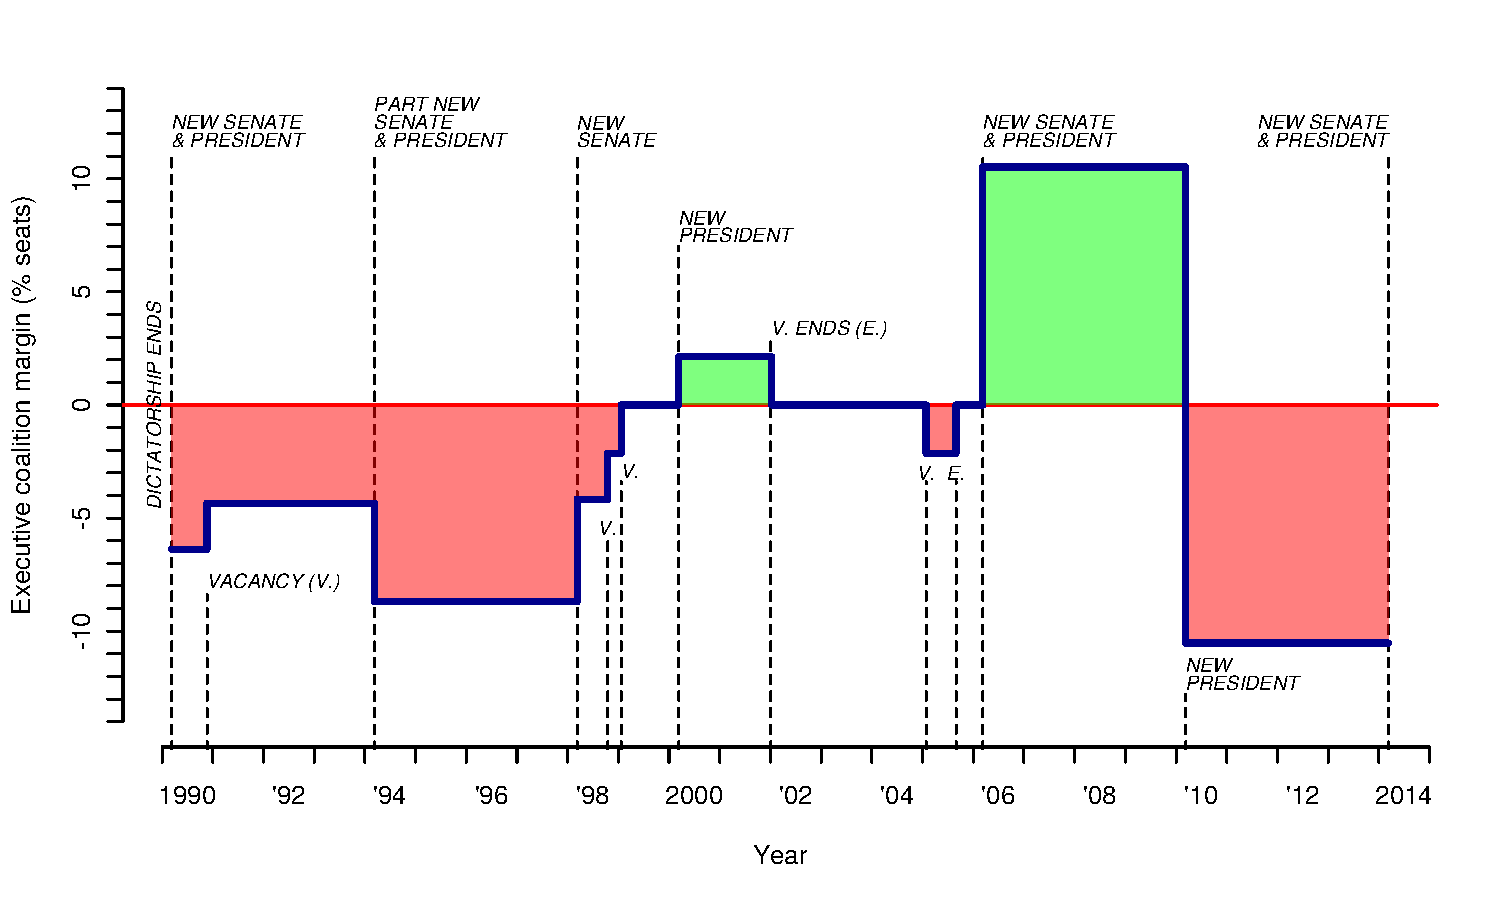
\includegraphics[width=\columnwidth]{../graphs/senChile.pdf}
  \caption{The Conservative chamber. The blue, crenellated line reports, longitudinally, the percentage of Senate seats controlled by the president's coalition minus the percentage controlled by the opposition. Totals include 38 elected senators and, up to 2006, 9 appointed senators and two or less senators for life. Vacancies, if any, are excluded from the denominator (see text). A new Senate is elected every eight years, and was partially renewed in 1994. Vacancies in the period: Ruiz Danyau, Air Force appointee, died in office 11/1990; Pinochet detained in London 10/1998; Errázuriz stripped of immunity 1/1999 (resinstated 1/2002); Lavandero stripped of immunity 1/2005 (replaced upon conviction 8/2005). }\label{f:senChile}
\end{center}
\end{figure}





% % \begin{tabular}{lrrrrrr}
% %                                   &  \mc{2}{c}{passed}    &  \mc{2}{c}{not}     &  \mc{2}{c}{all}      \\    
% % Bills with urgency in             &  N     &  \%          &  N     &  \%        &  N     &  \%         \\ \hline
% % $1^{st}$ chamber only              &   122  &  \emph{32}   &   259  &  \emph{68} &   381  &  \emph{100} \\
% % $2^{nd}$ chamber only              &   129  &  \emph{68}   &    62  &  \emph{32} &   191  &  \emph{100} \\
% % conference only                   &    27  &  \emph{82}   &     6  &  \emph{18} &    33  &  \emph{100} \\
% % $1^{st}$ and $2^{nd}$               &   363  &  \emph{81}   &    87  &  \emph{19} &   450  &  \emph{100} \\
% % $1^{st}$ and conference            &    39  &  \emph{93}   &     3  &  \emph{7}  &    42  &  \emph{100} \\
% % $2^{nd}$ and conference            &    37  &  \emph{90}   &     4  &  \emph{10} &    41  &  \emph{100} \\
% % $1^{st}$, $2^{nd}$, and conference  &   212  &  \emph{94}   &    14  &  \emph{6}  &   226  &  \emph{100} \\
% % no urgency                        &   541  &  \emph{10}   &  5097  &  \emph{90} &   5638 &  \emph{100} \\ \hline
% % %total                             &   929  &  \emph{68}   &   435  &  \emph{32} &  1364  &  \emph{100} \\ \hline
% % \end{tabular}

% An urgency message can be sent at any stage of the bicameral legislative process, compelling the chamber receiving it to act on a bill. Since urgencies expire once the chamber has finished, it is not uncommon for presidents to send messages at more than one step. Two-fifths of bills with urgencies were deemed so in two or three steps of the legislative process---the first chamber, the second, and/or the bicameral conference.    

% % \begin{table}
% % \begin{center}
% % \begin{tabular}{lrrr|rrr}
% %                                   &  \mc{6}{c}{Proposer}                                               \\    
% %                                   &  \mc{3}{c}{president}         &  \mc{3}{c}{member of Congress}             \\    
% % Bills with urgency in             &  \% pass   & \% not    & ~~~~~N &  \% pass  & \% not    & ~~~~~N \\ \hline
% % $1^{st}$ chamber only              &  \emph{40} & \emph{60} & 278  & \emph{12} & \emph{88} & 103  \\
% % $2^{nd}$ chamber only              &  \emph{84} & \emph{16} &  98  & \emph{51} & \emph{49} &  93  \\
% % conference only                   &  \emph{95} & \emph{5}  &  20  & \emph{62} & \emph{38} &  13  \\
% % $1^{st}$ and $2^{nd}$               &  \emph{86} & \emph{14} & 369  & \emph{58} & \emph{42} &  81  \\
% % $1^{st}$ and conference            &  \emph{92} & \emph{8}  &  39  & \emph{100}& \emph{0}  &   3  \\
% % $2^{nd}$ and conference            &  \emph{100}& \emph{0}  &  18  & \emph{83} & \emph{17} &  23  \\
% % $1^{st}$, $2^{nd}$, and conference  &  \emph{94} & \emph{6}  & 192  & \emph{91} & \emph{9}  &  34  \\
% % no urgency                        &  \emph{67} & \emph{33} & 455  & \emph{5}  & \emph{95} & 5183  \\ \hline
% % \end{tabular}
% % \caption{The legislative process, urgency messages, and bill passage by proposer 1998--2014}\label{T:stepsUrgencyPass}
% % \end{center}
% % \end{table}

% \begin{table}
% \begin{center}
% \begin{tabular}{lrrr|rrr}
%                        &  \mc{6}{c}{Proposer}                                               \\    
% Step(s) with           &  \mc{3}{c}{president}         &  \mc{3}{c}{member of Congress}             \\    
% urgency declared       &  \% pass    & \% not      & ~~~~~N &  \% pass  & \% not      & ~~~~~N \\ \hline
% 1 only                 &  \emph{41}  &  \emph{59}  &  285 &  \emph{12}  &  \emph{88}  &  103 \\
% 2 only                 &  \emph{84}  &  \emph{16}  &  102 &  \emph{52}  &  \emph{48}  &  96  \\
% 3 only                 &  \emph{90}  &  \emph{10}  &  10  &  \emph{75}  &  \emph{25}  &  4   \\
% $c$ only               &  \emph{100} &  \emph{0}   &  8   &  \emph{57}  &  \emph{43}  &  7   \\
% 1 and 2                &  \emph{85}  &  \emph{15}  &  382 &  \emph{60}  &  \emph{40}  &  84  \\
% two of more            &  \emph{100} &  \emph{0}   &  37  &  \emph{90}  &  \emph{10}  &  21  \\
% 1, 2, and 3            &  \emph{94}  &  \emph{6}   &  89  &  \emph{90}  &  \emph{10}  &  10  \\
% three of more          &  \emph{96}  &  \emph{4}   &  55  &  \emph{86}  &  \emph{14}  &  14  \\
% 1, 2, 3, and $c$       &  \emph{93}  &  \emph{7}   &  44  &  \emph{80}  &  \emph{20}  &  10  \\
% no urgency             &  \emph{67}  &  \emph{33}  &  457 &  \emph{5}   &  \emph{95}  &  5184 \\ \hline
% \end{tabular}
% \caption{Legislative steps, urgency messages, and bill passage by proposer 1998--2014. Steps are coded thus: 1 for the chamber of origin, 2 for the revising chamber, 3 for the chamber of origin's response, and $c$ for the conference committee. Cells report bill frequencies.}\label{T:stepsUrgencyPass}
% \end{center}
% \end{table}






\begin{sidewaysfigure}
\begin{tabular}{cc}
%\textbf{Executive-initiated bills} & \textbf{MC-initiated bills} \\
\textbf{Piñera bills sent to Deputies} & \textbf{Piñera bills sent to Senate} \\
($N=314$) & ($N=90$) \\
\tikzstyle{mid}=[circle,draw]
\tikzstyle{middot}=[circle,draw,dashed]
\begin{tikzpicture}[shorten >=1pt,node distance=2cm,auto,scale=.6]
%\draw[help lines] (-6,-6) grid (6,6);
\node at (-4,6) (st) {\footnotesize{\textbf{\texttt{start}}}};
\node[mid]     at (0,0)   (p)  {\textbf{Exec.}};
\node[mid,green] at (0,6)   (n1) {\textbf{Orig.}};
\node[mid,red]   at (6,0)   (n2) {\textbf{Rev.}};
\node[mid,green] at (0,-6)  (n3) {\textbf{Orig.}};
\node[mid]       at (-6,0)  (c)  {\textbf{Conf.}};
%\node[middot]    at (2,3)   (u)  {$u$};
%\node[middot]    at (3,-2)  (v)  {$u$};
%\node[middot]    at (-2,-3) (w)  {$u$};
%\node[middot]    at (-3,2)  (x)  {$u$};
\draw [-stealth] (st)                    edge node {100} (n1);
\draw [-stealth] (n1) [loop above]       edge node              {22} ();    % l11 $A$
%\draw [-stealth] (n1) [bend left,dashed] edge node              {75} (u);   % l1u $B$
\draw [-stealth] (n1) [out=0,in=90]      edge node              {78} (n2);  % l12 $C$
%\draw [-stealth] (u)  [bend left]        edge node              {14} (n1);  % lu1 $D$
%\draw [-stealth] (u)                     edge node              {61} (n2);  % lu2 $E$
\draw [-stealth] (n2) [loop right]       edge node              {10} ();    % l22 $F$
\draw [-stealth] (n2) [out=-90,in=0]     edge node              {31} (n3);  % l23 $G$
%\draw [-stealth] (n2) [bend left,dashed] edge node              {57} (v);   % l2v $H$
\draw [-stealth] (n2) [out=170, in=10]   edge node [swap]       {36} (p);   % l2p $I$
%\draw [-stealth] (v)  [bend left]        edge node              { 7} (n2);  % lv2 $J$
%\draw [-stealth] (v)                     edge node [swap]       {24} (p)    % lvp $K$
%                 (v)                     edge node              {25} (n3);  % lv3 $L$
\draw [-stealth] (n3) [loop below]       edge node              { 0} ();    % l33 $N$
\draw [-stealth] (n3) [out=180,in=-90]   edge node              { 7} (c);   % l3c $O$
%\draw [-stealth] (n3) [bend left,dashed] edge node              {11} (w);   % l3w $P$
\draw [-stealth] (n3) [out=80, in=-80]   edge node [swap]       {24} (p);   % l3p $Q$
%\draw [-stealth] (w)  [bend left]        edge node [near start] { 0} (n3);  % lw3 $R$
%\draw [-stealth] (w)                     edge node              { 9} (p)    % lwp $S$
%                 (w)                     edge node              { 1} (c);   % lwc $U$
\draw [-stealth] (c)  [loop left]        edge node              { 0} ();    % lcc $V$
%\draw [-stealth] (c)  [bend left,dashed] edge node              { 5} (x);   % lcx $W$
\draw [-stealth] (c)  [out=-10, in=-170] edge node [swap]       { 7} (p);   % lcp $X$
%\draw [-stealth] (x)  [bend left]        edge node              { 0} (c);   % lxc $Y$
%\draw [-stealth] (x)                     edge node              { 5} (p);   % lcp $Z$
\end{tikzpicture}
&
\tikzstyle{mid}=[circle,draw]
\tikzstyle{middot}=[circle,draw,dashed]
\begin{tikzpicture}[shorten >=1pt,node distance=2cm,auto,scale=.6]
%\draw[help lines] (-6,-6) grid (6,6);
\node at (-4,6) (st) {\footnotesize{\textbf{\texttt{start}}}};
\node[mid]       at (0,0)   (p)  {\textbf{Exec.}};
\node[mid,red]   at (0,6)   (n1) {\textbf{Orig.}};
\node[mid,green] at (6,0)   (n2) {\textbf{Rev.}};
\node[mid,red]   at (0,-6)  (n3) {\textbf{Orig.}};
\node[mid]       at (-6,0)  (c)  {\textbf{Conf.}};
%\node[middot]    at (2,3)   (u)  {$u$};
%\node[middot]    at (3,-2)  (v)  {$u$};
%\node[middot]    at (-2,-3) (w)  {$u$};
%\node[middot]    at (-3,2)  (x)  {$u$};
\draw [-stealth] (st)                    edge node {100} (n1);
\draw [-stealth] (n1) [loop above]       edge node              {39} ();    % l11 $A$
%\draw [-stealth] (n1) [bend left,dashed] edge node              {79} (u);   % l1u $B$
\draw [-stealth] (n1) [out=0,in=90]      edge node              {61} (n2);  % l12 $C$
%\draw [-stealth] (u)  [bend left]        edge node              {31} (n1);  % lu1 $D$
%\draw [-stealth] (u)                     edge node              {48} (n2);  % lu2 $E$
\draw [-stealth] (n2) [loop right]       edge node              { 7} ();    % l22 $F$
\draw [-stealth] (n2) [out=-90,in=0]     edge node              {29} (n3);  % l23 $G$
%\draw [-stealth] (n2) [bend left,dashed] edge node              {47} (v);   % l2v $H$
\draw [-stealth] (n2) [out=170, in=10]   edge node [swap]       {26} (p);   % l2p $I$
%\draw [-stealth] (v)  [bend left]        edge node              { 6} (n2);  % lv2 $J$
%\draw [-stealth] (v)                     edge node [swap]       {18} (p)    % lvp $K$
%                 (v)                     edge node              {23} (n3);  % lv3 $L$
\draw [-stealth] (n3) [loop below]       edge node              { 0} ();    % l33 $N$
\draw [-stealth] (n3) [out=180,in=-90]   edge node              {11} (c);   % l3c $O$
%\draw [-stealth] (n3) [bend left,dashed] edge node              {18} (w);   % l3w $P$
\draw [-stealth] (n3) [out=80, in=-80]   edge node [swap]       {18} (p);   % l3p $Q$
%\draw [-stealth] (w)  [bend left]        edge node [near start] { 0} (n3);  % lw3 $R$
%\draw [-stealth] (w)                     edge node              {11} (p)    % lwp $S$
%                 (w)                     edge node              { 7} (c);   % lwc $U$
\draw [-stealth] (c)  [loop left]        edge node              { 2} ();    % lcc $V$
%\draw [-stealth] (c)  [bend left,dashed] edge node              { 8} (x);   % lcx $W$
\draw [-stealth] (c)  [out=-10, in=-170] edge node [swap]       { 9} (p);   % lcp $X$
%\draw [-stealth] (x)  [bend left]        edge node              { 1} (c);   % lxc $Y$
%\draw [-stealth] (x)                     edge node              { 7} (p);   % lcp $Z$
\end{tikzpicture}
\\
\end{tabular}
\caption{Bills' paths in the legislative process compact}
\end{sidewaysfigure}





\begin{sidewaysfigure}
\begin{tabular}{cc}
%\textbf{Executive-initiated bills} & \textbf{MC-initiated bills} \\
\textbf{Piñera bills sent to Deputies} & \textbf{Piñera bills sent to Senate} \\
($N=314$) & ($N=90$) \\
\tikzstyle{mid}=[circle,draw]
\tikzstyle{middot}=[circle,draw,dashed]
\begin{tikzpicture}[shorten >=1pt,node distance=2cm,auto,scale=.6]
%\draw[help lines] (-6,-6) grid (6,6);
\node at (-4,6) (st) {\footnotesize{\textbf{\texttt{start}}}};
\node[mid]     at (0,0)   (p)  {\textbf{Exec.}};
\node[mid,green] at (0,6)   (n1) {\textbf{Orig.}};
\node[mid,red]   at (6,0)   (n2) {\textbf{Rev.}};
\node[mid,green] at (0,-6)  (n3) {\textbf{Orig.}};
\node[mid]       at (-6,0)  (c)  {\textbf{Conf.}};
\node[middot]    at (2,3)   (u)  {$u$};
\node[middot]    at (3,-2)  (v)  {$u$};
\node[middot]    at (-2,-3) (w)  {$u$};
\node[middot]    at (-3,2)  (x)  {$u$};
\draw [-stealth] (st)                    edge node {100} (n1);
\draw [-stealth] (n1) [loop above]       edge node              { 8} ();    % l11 $A$
\draw [-stealth] (n1) [bend left,dashed] edge node              {75} (u);   % l1u $B$
\draw [-stealth] (n1) [out=0,in=90]      edge node              {17} (n2);  % l12 $C$
\draw [-stealth] (u)  [bend left]        edge node              {14} (n1);  % lu1 $D$
\draw [-stealth] (u)                     edge node              {61} (n2);  % lu2 $E$
\draw [-stealth] (n2) [loop right]       edge node              { 3} ();    % l22 $F$
\draw [-stealth] (n2) [out=-90,in=0]     edge node              { 6} (n3);  % l23 $G$
\draw [-stealth] (n2) [bend left,dashed] edge node              {57} (v);   % l2v $H$
\draw [-stealth] (n2) [out=170, in=10]   edge node [swap]       {12} (p);   % l2p $I$
\draw [-stealth] (v)  [bend left]        edge node              { 7} (n2);  % lv2 $J$
\draw [-stealth] (v)                     edge node [swap]       {24} (p)    % lvp $K$
                 (v)                     edge node              {25} (n3);  % lv3 $L$
\draw [-stealth] (n3) [loop below]       edge node              { 0} ();    % l33 $N$
\draw [-stealth] (n3) [out=180,in=-90]   edge node              { 6} (c);   % l3c $O$
\draw [-stealth] (n3) [bend left,dashed] edge node              {11} (w);   % l3w $P$
\draw [-stealth] (n3) [out=80, in=-80]   edge node [swap]       {15} (p);   % l3p $Q$
\draw [-stealth] (w)  [bend left]        edge node [near start] { 0} (n3);  % lw3 $R$
\draw [-stealth] (w)                     edge node              { 9} (p)    % lwp $S$
                 (w)                     edge node              { 1} (c);   % lwc $U$
\draw [-stealth] (c)  [loop left]        edge node              { 0} ();    % lcc $V$
\draw [-stealth] (c)  [bend left,dashed] edge node              { 5} (x);   % lcx $W$
\draw [-stealth] (c)  [out=-10, in=-170] edge node [swap]       { 2} (p);   % lcp $X$
\draw [-stealth] (x)  [bend left]        edge node              { 0} (c);   % lxc $Y$
\draw [-stealth] (x)                     edge node              { 5} (p);   % lcp $Z$
\end{tikzpicture}
&
\tikzstyle{mid}=[circle,draw]
\tikzstyle{middot}=[circle,draw,dashed]
\begin{tikzpicture}[shorten >=1pt,node distance=2cm,auto,scale=.6]
%\draw[help lines] (-6,-6) grid (6,6);
\node at (-4,6) (st) {\footnotesize{\textbf{\texttt{start}}}};
\node[mid]       at (0,0)   (p)  {\textbf{Exec.}};
\node[mid,red]   at (0,6)   (n1) {\textbf{Orig.}};
\node[mid,green] at (6,0)   (n2) {\textbf{Rev.}};
\node[mid,red]   at (0,-6)  (n3) {\textbf{Orig.}};
\node[mid]       at (-6,0)  (c)  {\textbf{Conf.}};
\node[middot]    at (2,3)   (u)  {$u$};
\node[middot]    at (3,-2)  (v)  {$u$};
\node[middot]    at (-2,-3) (w)  {$u$};
\node[middot]    at (-3,2)  (x)  {$u$};
\draw [-stealth] (st)                    edge node {100} (n1);
\draw [-stealth] (n1) [loop above]       edge node              { 8} ();    % l11 $A$
\draw [-stealth] (n1) [bend left,dashed] edge node              {79} (u);   % l1u $B$
\draw [-stealth] (n1) [out=0,in=90]      edge node              {13} (n2);  % l12 $C$
\draw [-stealth] (u)  [bend left]        edge node              {31} (n1);  % lu1 $D$
\draw [-stealth] (u)                     edge node              {48} (n2);  % lu2 $E$
\draw [-stealth] (n2) [loop right]       edge node              { 1} ();    % l22 $F$
\draw [-stealth] (n2) [out=-90,in=0]     edge node              { 6} (n3);  % l23 $G$
\draw [-stealth] (n2) [bend left,dashed] edge node              {47} (v);   % l2v $H$
\draw [-stealth] (n2) [out=170, in=10]   edge node [swap]       { 8} (p);   % l2p $I$
\draw [-stealth] (v)  [bend left]        edge node              { 6} (n2);  % lv2 $J$
\draw [-stealth] (v)                     edge node [swap]       {18} (p)    % lvp $K$
                 (v)                     edge node              {23} (n3);  % lv3 $L$
\draw [-stealth] (n3) [loop below]       edge node              { 0} ();    % l33 $N$
\draw [-stealth] (n3) [out=180,in=-90]   edge node              { 4} (c);   % l3c $O$
\draw [-stealth] (n3) [bend left,dashed] edge node              {18} (w);   % l3w $P$
\draw [-stealth] (n3) [out=80, in=-80]   edge node [swap]       { 7} (p);   % l3p $Q$
\draw [-stealth] (w)  [bend left]        edge node [near start] { 0} (n3);  % lw3 $R$
\draw [-stealth] (w)                     edge node              {11} (p)    % lwp $S$
                 (w)                     edge node              { 7} (c);   % lwc $U$
\draw [-stealth] (c)  [loop left]        edge node              { 1} ();    % lcc $V$
\draw [-stealth] (c)  [bend left,dashed] edge node              { 8} (x);   % lcx $W$
\draw [-stealth] (c)  [out=-10, in=-170] edge node [swap]       { 2} (p);   % lcp $X$
\draw [-stealth] (x)  [bend left]        edge node              { 1} (c);   % lxc $Y$
\draw [-stealth] (x)                     edge node              { 7} (p);   % lcp $Z$
\end{tikzpicture}
\\
\end{tabular}
\caption{Bills' paths in the legislative process. Orig.\ and Rev.\ are the originating and revising chambers, respectively, Conf.\ the conference committee, and Exec.\ the executive. Numbers are relative to base 100 (ie., frequency*100/total bills), rounded to nearest integer.}\label{F:billPaths}
\end{sidewaysfigure}



% \section{Discussion}

% The more difficult it is for an assembly to form and maintain majorities capable of passing legislation, the more attractive it becomes to delegate responsibility to the executive.  Specific examples of situations where decrees may become more attractive are systems where legislative parties have a chronic incapacity to discipline members (as in Brazil), or bicameral systems where malapportionment typically produces majorities of different parties in each house, as in Chile before the removal of appointed senators in 2006 \citep[see][]{carey.shugart.1998a,cox.mccubbins.2001}.

% A theme worth pursuing are the determinants of unilateralism.  The logic behind executive vetoes (a concurrent consent institution) extends naturally to executive decrees (a restricted unilateralism institution). In the Linzian framework,\footnote{``[T]here is no democratic principle to resolve [conflict]'' \citeyear[][7]{linz.1994}.} unilateralism appears as unconstitutional moves by the executive to bypass the legislature in the context of impasse---an indicator of deep polarization (also O'Donnell). Presidential unilateralism is tantamount to a democratic system overheating dangerously, perhaps ready to melt into authoritarianism.  The factor driving decree incidence is, again, polarization between the branches. Is there evidence? 

% Because it pays attention to a single case giving no constitutional decree authority to its president, Cameron's work remains silent about executive unilateralism.  But following the logic of the bargaining approach, decrees should simply represent one additional tool that the president can resort to in his or her quest for influence on policy.  The veto power has a ``second face'' pointing to silent influence through a capacity of players to anticipate each other's acts; uncertainty reduces that capacity, prompting mistakes and a strategic use of them to gain reputations of toughness in bargaining \citep{cameron.2000,mccarty.1997}.  In the same fashion the decree power hides a second face (e.g. Congress makes a slightly larger concession to the president to avoid a decree of his or hers), and to the extent that players have incomplete information, some should occur and be rescinded as mistakes and reputation-building maneuvers.  

% Decrees can also be construed as part of a position-taking game.  It seems plausible that a president decrees some policy knowing, beforehand, that it will be rescinded by the assembly.  The intention is to force the assembly to reject policy popular to his constituents, increase the salience of the issue, and subsequently exploit this when campaigning (or give fellow party members a banner to fly in their campaigns).  Similarly, the assembly may concoct a bill attempting to avoid an executive decree modifying it; in doing so it may miscalculate and make insufficient concessions to the president, prompting the decree which legislators meant to avoid.  



\section{Conclusion}

Promising line of research?

``Can have dramatic effects on executive-legislative relations, legislative organization, and the policy process more generally'' (Morgenstern) 

%Simplification is understandable in the spirit of parsimony. Other things constant, a simpler, more general theory is better. But omitting detail has, in this case, not been conducive to a better understanding of decision-making in systems of separation of power. 

% It does create new opportunities for negotiation between the branches. open very interesting strategic angles new dimensions in bargaining. 

% None helps end gridlock, but puts pressure on legislature --- must act, must postpone other priorities. 








\bibliographystyle{apsr}
\bibliography{/home/eric/Dropbox/mydocs/magar}

\end{document}

